\documentclass[a4paper, 11pt,reqno]{article}
\input{macro/package.tex}
\input{macro/environement}
% Header et footer

\pagestyle{fancy}
\fancyhead{}
\fancyfoot{}
\renewcommand{\headwidth}{\textwidth}
\renewcommand{\footrulewidth}{0.4pt}
\renewcommand{\headrulewidth}{0pt}
\renewcommand{\footruleskip}{5px}

\fancyfoot[R]{Olivier Glorieux}
%\fancyfoot[R]{Jules Glorieux}

\fancyfoot[C]{ Page \thepage }
\fancyfoot[L]{1BIOA - Lycée Chaptal}
%\fancyfoot[L]{MP*-Lycée Chaptal}
%\fancyfoot[L]{Famille Lapin}

\input{macro/newcommand.tex}
\geometry{hmargin=1.0cm, vmargin=2.5cm}


\newcommand{\type}{TD }
\excludecomment{correction}
%\newcommand{\type}{Correction TD }


\begin{document}

\title{\type 18 : DL}
% debut
%------------------------------------------------


\vspace{0.2cm}
\section{Négligeabilité}

\begin{exercice}
	Classer les fonctions suivantes par ordre de négligeabilité en $+\infty$:
	$$f_1(x)=x,\ f_2(x)=\exp(x),\ f_3(x)=\frac 1x,\ f_4(x)=2,\ f_5(x)=\ln(x),\ f_6(x)=\sqrt x\ln x,\ f_7(x)=\frac{e^x}{\sqrt x}.$$
\end{exercice}

\begin{correction}
	A Venir
\end{correction}

\begin{exercice}
	Classer les fonctions suivantes par ordre de négligeabilité en $0$:
	$$f_1(x)=x,\ f_2(x)=\exp(x^2)-1,\ f_3(x)=\frac 1x,\ f_4(x)=x\sqrt{x},\ f_5(x)=\ln(x),\ f_6(x)=\sqrt x\ln x,\ f_7(x)=\ln(x+1).$$
\end{exercice}

\begin{correction}
	A Venir
\end{correction}

\begin{exercice}
	Soit $f$ et $g$ deux fonctions. Montrer que
	$$f(x)\equivalent{+\infty} g(x)  \equivaut f(x)-g(x)=o(g(x))$$
\end{exercice}
\begin{correction}
	A Venir
\end{correction}

\begin{exercice}
	Soit $f(x)= \sqrt{x+1}$ et $g(x)=\sqrt{x}$
	\begin{enumerate}
		\item Montrer que $f(x)\equivalent{+\infty} g(x)$
		\item Déterminer $\alpha \in \R$ tel que
		      $$ f(x) -g(x) =\frac{1}{x^\alpha} + o\left(\frac{1}{x^\alpha} \right)$$
	\end{enumerate}

\end{exercice}
\begin{correction}
	A Venir
\end{correction}
%--------------------------------------------------
%--------------------------------------------------
\noindent\section{\large{Calculs de d\'eveloppements limit\'es}}
%-----------------------------------------------

\begin{exercice}  \;
	Dans chacun des cas suivants, d\'eterminer le d\'eveloppement limit\'e de la fonction $f$ au voisinage de 0 \`a l'ordre donn\'e:
	\begin{enumerate}
		\begin{minipage}[t]{0.45\textwidth}
			\item $f(x)=e^x-\ddp\frac{1}{1-x}$ \`a l'ordre 2\vsec
			\item $f(x)=\exp{(\sin{x})}$ \`a l'ordre 4\vsec
			\item $f(x)=\sqrt[3]{1+x+x^2}$ \`a l'ordre 2\vsec
			\item $f(x)=\cos{\sqrt{x}}$ \`a l'ordre 5\vsec
			\item $f(x)=\ddp\frac{1}{x}-\ddp\frac{1}{\sin{x}}$ \`a l'ordre 1\vsec
			\item $f(x)=(\cos{x})^{\sin{x}}$ \`a l'ordre 5\vsec
			\item $f(x)=(1+x)^{\frac{1}{x}}$ \`a l'ordre 2\vsec
			\item $f(x)=\sin{x}-x\cos{x}$ \`a l'ordre 8\vsec
			\item $f(x)=2^x-1$ \`a l'ordre 2 \vsec
			\item $f(x)=e^{\sqrt{1+x}}$ \`a l'ordre 3\vsec
		\end{minipage}
		\quad
		\begin{minipage}[t]{0.45\textwidth}
			\item $f(x)=\tan^2{x}$ \`a l'ordre 6\vsec
			\item $f(x)=\ln{\left( \ddp\frac{\sin{x}}{x} \right)}$ \`a l'ordre 4\vsec
			\item $f(x)=\ddp\frac{1+x}{(1-x)^3}$ \`a l'ordre 3\vsec
			\item $f(x)=\ln{(1+\cos{(2x)})}$ \`a l'ordre 4\vsec
			\item $f(x)=\ddp\frac{x+1}{x^2+x+2}$ \`a l'ordre 3\vsec
			\item $f(x)=\left(\ddp\frac{\sin{x}}{x}  \right)^2$ \`a l'ordre 4\vsec
			\item $f(x)=\cos{\left( \ddp\frac{\pi}{2}\ddp\frac{x}{\tan{x}} \right)}$ \`a l'ordre 4\vsec
			\item $f(x)=\left(1+\arctan{x}\right)^{\frac{1}{x}}$ \`a l'ordre 3\vsec
			%\item $f(x)=\arcsin{\left( \ln{(\cos{x})}\right)}$ \`a l'ordre 4\vsec
		\end{minipage}
	\end{enumerate}
\end{exercice}
\begin{correction}  \;
	\begin{enumerate}
		\item \textbf{DL en $0$ \`a l'ordre $2$ de $\mathbf{f(x)=e^x-\ddp\frac{1}{1-x}}$ :}\\
		      On \'ecrit chacun des DL et on fait la somme :
		      $$f(x) \underset{0}{=}  1+x+\frac{x^2}{2}+o(x^2) - (1+x+x^2+o(x^2)) = -\frac{x^2}{2} + o(x^2).$$
		      On obtient donc : \fbox{$f(x)\underset{0}{=} -\ddp\frac{x^2}{2}  + o(x^2)$}.\\
		      On en d\'eduit que la tangente en $0$ a pour \'equation $y=0$, et comme $-\ddp\frac{x^2}{2}<0$, $\mathcal{C}_f$ est en dessous de sa tangente au voisinage de $0$.
		      %-------------------------------------------------
		\item \textbf{DL en $0$ \`a l'ordre 4 de $\mathbf{f(x)=\exp{(\sin{x})}}$ :}\\
		      On a, en \'ecrivant le $DL_4(0)$ de la fonction sinus :
		      $$f(x) \underset{0}{=}  \exp\left( x-\frac{x^3}{3!} + o(x^4)\right).$$
		      On pose $u(x) = \ddp x-\frac{x^3}{3!} + o(x^4)$. Comme $u(x) \mathop{\rightarrow}\limits_{x\to 0} 0$, on peut composer les DL. On a :
		      $$e^u \underset{0}{=} 1+u+\frac{u^2}{2} + \frac{u^3}{3!} + \frac{u^4}{4!} + o(u^4)$$
		      donc on en d\'eduit :
		      $$\begin{array}{rcl}
				      f(x) & \underset{0}{=} & \ddp 1 + x-\frac{x^3}{3!} + \frac{\left(x-\frac{x^3}{3!}\right)^2}{2} + \frac{\left(x-\frac{x^3}{3!}\right)^3}{3!} + \frac{\left(x-\frac{x^3}{3!}\right)^4}{4!} + o(x^4)\vsec \\
				           & \underset{0}{=} & \ddp 1 + x-\frac{x^3}{3!} + \frac{x^2}{2} - 2 \times \frac{x^4}{2\times 3!} + \frac{x^3}{3!} + \frac{x^4}{4!} + o(x^4)
			      \end{array}
		      $$
		      Soit : \fbox{$f(x)\underset{0}{=} 1+x+\ddp\frac{x^2}{2}-\ddp\frac{x^4}{8} + o(x^4)$}.\\
		      On en d\'eduit que la tangente en $0$ a pour \'equation $y=1+x$, et comme $\ddp\frac{x^2}{2}>0$, $\mathcal{C}_f$ est au dessus de sa tangente au voisinage de $0$.
		      %-------------------------------------------------
		\item \textbf{DL en $0$  \`a l'ordre 2 de $\mathbf{f(x)=\sqrt[3]{1+x+x^2}}$:}\\
		      On pose $u(x) = x+x^2$. Comme $u(x) \mathop{\rightarrow}\limits_{x\to 0} 0$, on peut composer les DL. On a :
		      $$(1+u)^{\frac{1}{3}} \underset{0}{=} 1+\frac{1}{3} u + \frac{\frac{1}{3}\left(\frac{1}{3}-1\right)}{2} u^2 + o(u^2),$$
		      donc on en d\'eduit :
		      $$f(x) \underset{0}{=} 1+\frac{1}{3} (x+x^2) - \frac{1}{9} (x+x^2)^2 + o(x^2) = 1 + \frac{1}{3} x + \frac{1}{3} x^2 - \frac{1}{9} x^2 +o(x^2).$$
		      Soit finalement : \fbox{$f(x) \underset{0}{=} 1+\ddp\frac{x}{3}+\ddp\frac{2}{9}x^2 + o (x^2)$}.\\
		      On en d\'eduit que la tangente en $0$ a pour \'equation $y=1+\ddp\frac{x}{3}$, et comme $\ddp\frac{2}{9}x^2>0$, $\mathcal{C}_f$ est au dessus de sa tangente au voisinage de $0$.
		      %-------------------------------------------------
		\item \textbf{DL en $0$  \`a l'ordre 5 de $\mathbf{f(x)=\cos{\sqrt{x}}}$:}\\
		      On pose $u(x) = \sqrt{x}$. On a bien $u(0)=0$, on peut donc composer. On \'ecrit le DL de $\cos$ \`a l'ordre $10$, afin d'obtenir de l'ordre $5$ en rempla\c cant $u$ par $\sqrt{x}$. On a :
		      $$\cos u \underset{0}{=} 1-\frac{u^2}{2}+\ddp\frac{u^4}{4!}-\ddp\frac{u^6}{6!}+\ddp\frac{u^8}{8!}-\ddp\frac{u^{10}}{10!}     + o (u^{10}),$$
		      soit en composant : \fbox{$f(x)\underset{0}{=} 1-\ddp\frac{x}{2}+\ddp\frac{x^2}{4!}-\ddp\frac{x^3}{6!}+\ddp\frac{x^4}{8!}-\ddp\frac{x^5}{10!}     + o (x^5)$}.\\
		      On en d\'eduit que la tangente en $0$ a pour \'equation $y=1-\ddp\frac{x}{2}$, et comme $\ddp\frac{x^2}{4!}>0$, $\mathcal{C}_f$ est au dessus de sa tangente au voisinage de $0$.
		      %-------------------------------------------------
		\item \textbf{DL en $0$ \`a l'ordre 1 de $\mathbf{f(x)=\ddp\frac{1}{x}-\ddp\frac{1}{\sin{x}}}$:}\\
		      On \'ecrit le DL de $\sin$ \`a l'ordre $3$ car il y a des simplifications :
		      $$\frac{1}{\sin x} \underset{0}{=} \frac{1}{x-\frac{x^3}{3!} + o(x^3)} \underset{0}{=}  \frac{1}{x\left(1-\frac{x^2}{3!}+o(x^2)\right)}.$$
		      On pose $u(x) = -\frac{x^2}{3!}+o(x^2)$. On a :
		      $$\frac{1}{1+u} \underset{0}{=} 1-u+o(u).$$
		      Comme $u(x) \mathop{\rightarrow}\limits_{x\to 0} 0$, on peut composer les DL:
		      $$\frac{1}{1-\frac{x^2}{3!}+o(x^2)}  \underset{0}{=}  1+\frac{x^2}{3!}+o(x^2)$$
		      et donc :
		      $$f(x) \underset{0}{=} \frac{1}{x} - \frac{1}{x} \left( 1+\frac{x^2}{3!}+o(x^2)\right),$$
		      soit finalement : \fbox{$f(x)\underset{0}{=} -\ddp\frac{x}{6}  + o (x)$}.\\
		      On en d\'eduit que la tangente en $0$ a pour \'equation $y= -\ddp\frac{x}{6}$. On ne conna\^it pas le terme suivant du DL, donc on ne peut pas d\'eterminer la position de $\mathcal{C}_f$ par rapport \`a sa tangente au voisinage de $0$ (il faudrait pousser le DL plus loin).
		      %-------------------------------------------------
		\item \textbf{DL en $0$ \`a l'ordre 5 de $\mathbf{f(x)=(\cos{x})^{\sin{x}}}$ :}\\
		      On commence par mettre la fonction sous forme exponentielle, car $\cos x >0$ au voisinage de $0$ : $f(x) = \exp(\sin x \ln (\cos x))$. On \'ecrit le DL de $\cos$ et on remplace dans le logarithme :
		      $$\ln(\cos x) \underset{0}{=} \ln\left(1-\frac{x^2}{2} + \frac{x^4}{4!} + o(x^4)\right).$$
		      On pose $u(x) \underset{0}{=} \ddp-\frac{x^2}{2} + \frac{x^4}{4!} + o(x^4)$.  Comme $u(x) \mathop{\rightarrow}\limits_{x\to 0} 0$, on peut composer les DL:
		      $$\ln(1+u) \underset{0}{=} u-\frac{u^2}{2} + \frac{u^3}{3}+o(u^3).$$
		      Soit par compos\?ee :
		      $$\begin{array}{rcl}
				      \ln(\cos x) & \underset{0}{=} & \ddp -\frac{x^2}{2} + \frac{x^4}{4!} - \frac{1}{2} \left(-\frac{x^2}{2} + \frac{x^4}{4!}\right)^2 + o(x^5) \vsec             \\
				                  & \underset{0}{=} & \ddp -\frac{x^2}{2} + \frac{x^4}{4!} -\frac{x^4}{8} + o(x^5) \; \underset{0}{=} \; -\frac{x^2}{2} - \frac{x^4}{12} + o(x^5).
			      \end{array}$$
		      On multiplie ensuite par le DL de $\sin$ :
		      $$\sin x \ln(\cos x) \underset{0}{=} \left(x-\frac{x^3}{3!} + \frac{x^5}{5!} + o(x^5)\right) \left(-\frac{x^2}{2} -\frac{x^4}{12} + o(x^5)\right) = - \frac{x^3}{2} - \frac{x^5}{12}+ \frac{x^5}{12}+o(x^5) = -\frac{x^3}{2} + o(x^5).$$
		      Puis on pose $u(x) = \ddp -\frac{x^3}{2} + o(x^5)$, et on compose par le DL de $\exp$ car $u(x) \mathop{\rightarrow}\limits_{x\to 0} 0$ :
		      \fbox{$f(x)\underset{0}{=} 1-\ddp\frac{x^3}{2}  +o(x^5)$}.\\
		      On en d\'eduit que la tangente en $0$ a pour \'equation $y=1$. De plus, on a  $-\ddp\frac{x^3}{2} >0$ si $x<0$, donc $\mathcal{C}_f$ est au dessus de sa tangente au voisinage de $0$ \`a gauche, et $-\ddp\frac{x^3}{2}<0$ si $x>0$, donc $\mathcal{C}_f$ est en dessous de sa tangente au voisinage de $0$ \`a droite.
		      %-------------------------------------------------
		\item \textbf{DL en $0$  \`a l'ordre 2 de $\mathbf{f(x)=(1+x)^{\frac{1}{x}}}$:}\\
		      On passe sous forme exponentielle : $f(x)=\exp(\frac{1}{x} \ln (1+x))$. On \'ecrit ensuite le $DL_3(0)$ de $\ln(1+x)$ et on divise par $x$ :
		      $$\frac{1}{x}\ln(1+x)\underset{0}{=} \frac{1}{x}\left( x-\frac{x^2}{2} + \frac{x^3}{3} + o(x^3)\right) \underset{0}{=} 1- \frac{x}{2}+\frac{x^2}{3} + o(x^2).$$
		      Attention on ne peut pas composer directement car ce qu'on obtient ne tend pas vers $0$ ! On remplace dans l'exponentielle :
		      $$f(x) \underset{0}{=} \exp\left( 1- \frac{x}{2}+\frac{x^2}{3} + o(x^2)\right) \underset{0}{=} e \times \exp \left(- \frac{x}{2}+\frac{x^2}{3} + o(x^2)\right).$$
		      On peut cette fois composer par le DL de $\exp$. On obtient :
		      $$f(x)  \underset{0}{=}  e\left( 1- \frac{x}{2}+\frac{x^2}{3} + \frac{x^2}{8} + o(x^2)\right)$$
		      Soit : \fbox{$f(x)\underset{0}{=} e\left(  1-\ddp\frac{x}{2}+\ddp\frac{11}{24}x^2    + o(x^2)\right)$}.\\
		      On en d\'eduit que la tangente en $0$ a pour \'equation $y=e-\ddp \frac{e}{2} x$, et comme $\ddp\frac{11}{24}x^2>0$, $\mathcal{C}_f$ est au dessus de sa tangente au voisinage de $0$.
		      %-------------------------------------------------
		\item \textbf{DL en $0$  \`a l'ordre 8 de $\mathbf{f(x)=\sin{x}-x\cos{x}}$:}\\
		      On \'ecrit les deux DL de $\sin$ et $\cos$ et on remet dans l'expression de $f$. On obtient :
		      \fbox{$f(x)\underset{0}{=} \ddp\frac{x^3}{3}-\ddp\frac{x^5}{30}+\ddp\frac{x^7}{840}    + o(x^8)$}.\\
		      On en d\'eduit que la tangente en $0$ a pour \'equation $y=0$. De plus, on a  $\ddp \frac{x^3}{3} < 0$ si $x<0$, donc $\mathcal{C}_f$ est en dessous de sa tangente au voisinage de $0$ \`a gauche, et $\ddp \frac{x^3}{3}>0$ si $x>0$, donc $\mathcal{C}_f$ est au dessus de sa tangente au voisinage de $0$ \`a droite.
		      %-------------------------------------------------
		\item \textbf{DL en $0$  \`a l'ordre 2 de $\mathbf{f(x)=2^x-1}$:} \\
		      On passe sous forme exponentielle : $f(x) = e^{x\ln2}-1$. On a $\lim\limits_{x\to 0} x\ln 2 =0$, donc on peut composer par le DL de $\exp$. On obtient :
		      \fbox{$f(x)\underset{0}{=} x\ln{2}+\ddp\frac{\ln^2{(2)}}{2}x^2  + o(x^2)$}.\\
		      On en d\'eduit que la tangente en $0$ a pour \'equation $y= x\ln{2}$, et comme $\ddp\frac{\ln^2{(2)}}{2}x^2 $, $\mathcal{C}_f$ est au dessus de sa tangente au voisinage de $0$.
		      %-------------------------------------------------
		\item \textbf{DL en $0$ \`a l'ordre 3 de $\mathbf{f(x)=e^{\sqrt{1+x}}}$ :}\\
		      On \'ecrit le DL de $\sqrt{1+x}$ :
		      $$\sqrt{1+x} \underset{0}{=} 1 + \frac{x}{2}- \frac{x^2}{8} + \frac{x^3}{16}  + o(x^3).$$
		      Attention, cette expression ne tend pas vers $0$, on ne peut pas composer directement. On remplace dans l'exponentielle :
		      $$f(x) \underset{0}{=} \exp\left(1 + \frac{x}{2}- \frac{x^2}{8} + \frac{x^3}{16} + o(x^3) \right) \underset{0}{=}  e \times \exp\left(\frac{x}{2}- \frac{x^2}{8} + \frac{x^3}{16} + o(x^3) \right) .$$
		      On peut cette fois composer, et on obtient :
		      $$f(x) \underset{0}{=} e \left(1+\frac{x}{2}- \frac{x^2}{8} + \frac{x^3}{16}+ \frac{1}{2} \left(\frac{x}{2}- \frac{x^2}{8} + \frac{x^3}{16}\right)^2 + \frac{1}{3!}\left(\frac{x}{2}- \frac{x^2}{8} + \frac{x^3}{16}\right)^3 + o(x^3) \right).$$
		      On en d\'eduit : \fbox{$f(x)\underset{0}{=} e\left( 1+\ddp\frac{x}{2}+\ddp\frac{x^3}{48}   + o(x^3)\right)$}.\\
		      On en d\'eduit que la tangente en $0$ a pour \'equation $y=e+\ddp \frac{e}{2} x$. De plus, on a  $\ddp\frac{x^3}{48} < 0$ si $x<0$, donc $\mathcal{C}_f$ est en dessous de sa tangente au voisinage de $0$ \`a gauche, et $\ddp\frac{x^3}{48}>0$ si $x>0$, donc $\mathcal{C}_f$ est au dessus de sa tangente au voisinage de $0$ \`a droite.%-------------------------------------------------
		\item \textbf{DL en $0$ \`a l'ordre 6 de $\mathbf{f(x)=\tan^2{x}}$ :}\\
		      On a $\ddp \tan x \underset{0}{=} x + \frac{x^3}{3} + \frac{2x^5}{15} + o(x^6).$
		      On \'el\`eve ce DL au carr\'e :
		      $$\tan x  \underset{0}{=} \left(x + \frac{x^3}{3} + \frac{2x^5}{15} + o(x^6)\right)^2 = x^2 + \frac{2 x^4}{3} + \frac{4x^6}{15} + \frac{x^6}{9} + o(x^6).$$
		      On obtient : \fbox{$f(x)\underset{0}{=} x^2+\ddp\frac{2}{3}x^4+\ddp\frac{17}{45}x^6   + o(x^6)$}.\\
		      On en d\'eduit que la tangente en $0$ a pour \'equation $y=0$, et comme $x^2>0$, $\mathcal{C}_f$ est au dessus de sa tangente au voisinage de $0$.
		      %-------------------------------------------------
		\item \textbf{DL en $0$ \`a l'ordre 3 de $\mathbf{f(x)=\ln{\left( \ddp\frac{\sin{x}}{x} \right)}}$ :}\\
		      On commence par \'ecrire le DL \`a l'int\'erieur :
		      $$\frac{\sin x}{x} \underset{0}{=} \frac{1}{x}\left(x- \frac{x^3}{3!} + o(x^4) \right) \underset{0}{=} 1 - \frac{x^2}{3!} + o(x^3).$$
		      On remplace dans le logarithme :
		      $$f(x) \underset{0}{=} \ln \left( 1 - \frac{x^2}{3!} + o(x^3)\right).$$
		      On pose $\ddp u(x) = - \frac{x^2}{3!} + o(x^3)$. On a bien $\lim\limits_{x\to 0 } u(x) = 0$, donc on peut composer par le DL du logarithme, et on obtient : \fbox{$f(x)\underset{0}{=} -\ddp\frac{x^2}{6}  + o(x^3)$}.\\
		      On en d\'eduit que la tangente en $0$ a pour \'equation $y=0$, et comme $-\ddp\frac{x^2}{6}<0$, $\mathcal{C}_f$ est en dessous de sa tangente au voisinage de $0$.
		      %-------------------------------------------------
		\item \textbf{DL en $0$  \`a l'ordre 3 de $\mathbf{f(x)=\ddp\frac{1+x}{(1-x)^3}}$:}\\
		      On a :
		      $$\frac{1}{1-x} \underset{0}{=} 1+x+x^2+x^3+o(x^3).$$
		      On \'el\`eve ce DL aa cube :
		      $$\frac{1}{(1-x)^3} \underset{0}{=} \left( 1+x+x^2+x^3+o(x^3) \right)^3 = 1+3x+3x^2+3x^3 + x^3 + 3x^2 +o(x^3) \underset{0}{=} 1+3x+6x^2+4x^3 + o(x^3) .$$
		      Puis on multiplie par $1+x$ :
		      $$f(x) \underset{0}{=} (1+x) \left(1+3x+6x^2+4x^3 + o(x^3)\right)  \underset{0}{=} 1+3x+6x^2+4x^3 + x + 3x^2+6x^3 + o(x^3).$$
		      Soit en rassemblant les termes : \fbox{$f(x)\underset{0}{=} 1+4x+9x^2+10x^3 + o(x^3)$}.\\
		      On en d\'eduit que la tangente en $0$ a pour \'equation $y=1+4x$, et comme $9x^2>0$, $\mathcal{C}_f$ est au dessus de sa tangente au voisinage de $0$.
		      %-------------------------------------------------
		\item \textbf{DL en $0$ \`a l'ordre 4 de $\mathbf{f(x)=\ln{(1+\cos{(2x)})}}$ :}\\
		      On commence par \'ecrire le DL de $\cos(2x)$ :
		      $$\cos(2x)\underset{0}{=} 1- \frac{(2x)^2}{2}+\frac{(2x)^4}{4!} + o(x^4) \underset{0}{=} 1-2x^2 + \frac{2x^4}{3} + o(x^4).$$
		      On remplace dans $f(x)$:
		      $$f(x) \underset{0}{=} \ln \left( 1 + 1-2x^2 + \frac{2x^4}{3} + o(x^4)\right)   \underset{0}{=} \ln \left(2-2x^2 + \frac{2x^4}{3} + o(x^4) \right).$$
		      Attention, on ne peut pas composer directement par le DL du logarithme :
		      $$f(x) \underset{0}{=} \ln 2 + \ln  \left(1-x^2 + \frac{x^4}{3} + o(x^4) \right) .$$
		      On compose ensuite les DL en posant $\ddp u(x) =-x^2 + \frac{x^4}{3} + o(x^4)$, qui tend bien vers $0$ en $0$, et on obtient :  \fbox{$f(x)\underset{0}{=} \ln{2}-x^2-\ddp\frac{x^4 }{6}  + o(x^4)$}.\\
		      On en d\'eduit que la tangente en $0$ a pour \'equation $y=\ln 2$, et comme $-x^20$, $\mathcal{C}_f$ est en dessous de sa tangente au voisinage de $0$.
		      %-------------------------------------------------
		\item \textbf{DL en $0$ \`a l'ordre 3 de $\mathbf{f(x)=\ddp\frac{x+1}{x^2+x+2}}$ :}\\
		      On essaye de se ramener \`a du $\ddp \frac{1}{1+u(x)}$, avec $u(x)$ qui tend vers $0$ en $0$ :
		      $$\frac{1}{x^2+x+2} = \frac{1}{2\left(1+\frac{x}{2}+ \frac{x^2}{2}\right)} = \frac{1}{2}\times  \frac{1}{1+\frac{x}{2}+ \frac{x^2}{2}}.$$
		      On pose $u(x) = \ddp  \frac{x}{2}+ \frac{x^2}{2}$, et on a bien $\lim\limits_{x \to 0} u(x) = 0$, on peut composer les DL :
		      $$\frac{1}{x^2+x+2}\underset{0}{=} \frac{1}{2}\left( 1- \left(\frac{x}{2}+ \frac{x^2}{2}\right) + \left(\frac{x}{2}+ \frac{x^2}{2}\right)^2 - \left(\frac{x}{2}+ \frac{x^2}{2}\right)^3 + o(x^3) \right).$$
		      En d\'eveloppant, puis en multipliant par $1+x$, on obtient : \fbox{$f(x)\underset{0}{=} \ddp\demi\left( 1+\ddp\frac{x}{2}-\ddp\frac{3x^2}{4}+\ddp\frac{x^3}{8}      \right) +o(x^3)$}.\\
		      On en d\'eduit que la tangente en $0$ a pour \'equation $y=\ddp\frac{1}{2}+\ddp\frac{x}{2}$, et comme $-\ddp\frac{3x^2}{8}<0$, $\mathcal{C}_f$ est en dessous de sa tangente au voisinage de $0$.
		      %-------------------------------------------------
		\item \textbf{DL en $0$ \`a l'ordre 4 de $\mathbf{f(x)=\left(\ddp\frac{\sin{x}}{x}  \right)^2}$ :}\\
		      On \'ecrit tout d'abord le DL \`a l'int\'erieur :
		      $$\frac{\sin x}{x} \underset{0}{=} \frac{1}{x}\left(x- \frac{x^3}{3!} + o(x^4) \right) \underset{0}{=} 1 - \frac{x^2}{3!} + o(x^3).$$
		      On \'el\`eve ensuite au carr\'e, et on obtient :
		      \fbox{$f(x)\underset{0}{=} 1-\ddp\frac{x^2}{3}+\ddp\frac{2}{45} x^4   + o (x^4)$}.\\
		      On en d\'eduit que la tangente en $0$ a pour \'equation $y=1$, et comme $-\ddp\frac{x^2}{3}<0$, $\mathcal{C}_f$ est en dessous de sa tangente au voisinage de $0$.
		      %-------------------------------------------------
		\item \textbf{DL en $0$ \`a l'ordre 4 de $\mathbf{f(x)=\cos{\left( \ddp\frac{\pi}{2}\ddp\frac{x}{\tan{x}} \right)}}$ :}\\
		      On commence par le DL \`a l'int\'erieur :
		      $$\frac{x}{\tan x} \underset{0}{=} \frac{x}{x+\frac{x^3}{3} + \frac{2x^5}{15} + o(x^5)} \underset{0}{=} \frac{1}{1+\frac{x^2}{3}+\frac{2x^4}{15}+o(x^4)}.$$
		      On pose ensuite $u(x) = \ddp \frac{x^2}{3}+\frac{2x^4}{15}$, qui tend vers $0$ en $0$. On peut donc composer les DL et on obtient :
		      $$\frac{x}{\tan x} \underset{0}{=} 1 - \left(\frac{x^2}{3}+\frac{2x^4}{15}\right) +  \left(\frac{x^2}{3}+\frac{2x^4}{15}\right)^2 + o(x^2)  \underset{0}{=} 1 - \frac{x^2}{3} + \frac{11x^4}{45}+o(x^4).$$
		      On remplace dans $f(x)$ :
		      $$f(x) \underset{0}{=} \cos\left(\frac{\pi}{2} \left(  1 - \frac{x^2}{3} + \frac{11x^4}{45}+o(x^4)\right) \right) \underset{0}{=} \sin \left(\frac{\pi}{6}x^2 - \frac{11\pi}{90}x^4 + o(x^4)\right)$$
		      en utilisant les formules de trigonom\'etrie. On a $\ddp \frac{\pi}{6}x^2 - \frac{11\pi}{90}x^4 + o(x^4)$ qui tend vers $0$ en $0$, donc on peut composer les DL, et on obtient :
		      \fbox{$f(x)\underset{0}{=} \ddp\frac{\pi}{6}x^2+\ddp\frac{\pi}{90} x^4   + o(x^4)$}.\\
		      On en d\'eduit que la tangente en $0$ a pour \'equation $y=0$, et comme $ \ddp\frac{\pi}{6}x^2>0$, $\mathcal{C}_f$ est au dessus de sa tangente au voisinage de $0$.
		      %-------------------------------------------------
		\item \textbf{DL en $0$  \`a l'ordre 3 de $\mathbf{f(x)=\left(1+\arctan{x}\right)^{\frac{1}{x}}}$:}\\
		      On met sous forme exponentielle : $f(x) = \exp\left(\frac{1}{x}\ln \left(1+\arctan x\right)\right)$. \\
		      On a de plus : $\ddp \arctan x = x - \frac{x^3}{3} + o(x^4)$, et donc on doit calculer le DL de :
		      $$ \ln(1+\arctan x) \underset{0}{=} \ln \left( 1 + x - \frac{x^3}{3} + o(x^4) \right).$$
		      On a $\ddp\lim\limits_{x \to 0} x - \frac{x^3}{3} + o(x^4) = 0$, donc par compos\'ee de DL :
		      $$\begin{array}{rcl}
				      \ln(1+\arctan x) & \underset{0}{=} & \ddp x - \frac{x^3}{3} - \frac{1}{2} \left( x - \frac{x^3}{3}\right)^2 + \frac{1}{3} \left( x - \frac{x^3}{3} \right)^3 - \frac{1}{4} \left( x - \frac{x^3}{3}\right)^4 + o(x^4)\vsec \\
				                       & \underset{0}{=} & \ddp x-\frac{x^2}{2} + \frac{x^4}{12} + o(x^4)
			      \end{array}$$
		      On obtient :
		      $$ f(x) \underset{0}{=} \exp\left(1-\frac{x}{2} + \frac{x^3}{12} + o(x^3)\right) \underset{0}{=} e\times \exp\left(-\frac{x}{2}+\frac{x^3}{12} + o(x^3)\right).$$
		      On a $\ddp\lim\limits_{x \to 0} -\frac{x}{2}+\frac{x^3}{12} + o(x^3) = 0$, donc par compos\'ee de DL :
		      $$\begin{array}{rcl}
				      \ddp f(x) & \underset{0}{=} & \ddp e\left(1+\left(-\frac{x}{2} + \frac{x^3}{12}\right) + \frac{1}{2}\left(-\frac{x}{2} + \frac{x^3}{12}\right)^2 + \frac{1}{6} \left(-\frac{x}{2} + \frac{x^3}{12}\right)^3 + o(x^3)\right)\vsec \\
				                & \underset{0}{=} & \ddp e\left( 1 - \frac{x}{2} + \frac{x^2}{8} + \frac{x^3}{16} + o(x^3)\right)
			      \end{array}$$
		      On obtient finalement :
		      \fbox{$f(x)\underset{0}{=} e-\ddp\frac{ex}{2}+\ddp\frac{ex^2}{8}+\ddp\frac{ex^3}{16}   + o(x^3)$}.\\
		      On en d\'eduit que la tangente en $0$ a pour \'equation $y=e-\ddp\frac{e}{2} x$, et comme $\ddp\frac{e x^2}{8}>0$, $\mathcal{C}_f$ est au dessus de sa tangente au voisinage de $0$.
		      %%-------------------------------------------------
		      %\item $f(x)=\arcsin{\left( \ln{(\cos{x})}\right)}$ \`a l'ordre 4\\
		      %\noindent $f(x)\underset{0}{=} -\ddp\frac{x^2}{2}+\ddp\frac{x^4}{6}   +\circ (x^4)$
		      %%------------------------
	\end{enumerate}
\end{correction}
%\vspace*{0.5cm}

%-----------------------------------------------
\begin{exercice}  \;
	D\'eterminer le d\'eveloppement limit\'e \`a l'ordre $n$ donn\'e de la fonction $f$ au voisinage de $x_0$ dans les cas suivants:
	\begin{enumerate}
		\item $f(x)=\sqrt{x}$ au voisinage de $x_0=\ddp\frac{1}{4}$ \`a l'ordre $n=5$\vsec
		\item $f(x)=\ddp\frac{1}{x}$ au voisinage de $x_0=1$ \`a l'ordre $n=5$\vsec
		\item $f(x)=\ddp\frac{x+1}{x-1}$ au voisinage de $x_0=3$ \`a l'ordre $n=4$\vsec
		\item $f(x)=\ddp\frac{\sin{x}}{\sqrt{x}}$ au voisinage de $x_0=\ddp\frac{\pi}{4}$ \`a l'ordre $n=3$\vsec
		\item $f(x)=x^{\frac{1}{-1+\ln{x}}}$ au voisinage de $x_0=1$ \`a l'ordre $n=3$\vsec
		\item $f(x)=e^{x-1}$ au voisinage de $x_0=1$ \`a l'ordre $n$ quelconque.\vsec
		      %\item $f(x)=\sin^2{\left( \ddp\frac{x}{2}\right)}$ au voisinage de $x_0=\ddp\frac{\pi}{3}$ \`a l'ordre $n=4$.
		      %\item $f(x)=\sqrt[3]{x^3+x^2}-\sqrt[3]{x^3-x^2}$ au voisinage de $x_0=+\infty$ \`a l'ordre $n=2$.
		\item $f(x)=\ddp\frac{x^n\ln{x}}{x^2-1}$ au voisinage de $x_0=1$ \`a l'ordre 2
	\end{enumerate}
\end{exercice}
\begin{correction}  \; Je ne donne les d\'etails que pour le d\'ebut.
	\begin{enumerate}
		\item \textbf{DL de $\mathbf{f(x)=\sqrt{x}}$ au voisinage de $\mathbf{x_0=\ddp\frac{1}{4}}$ \`a l'ordre $n=5$}.\\
		      On se ram\`ene \`a $0$ en posant $\ddp X=x-\frac{1}{4}$, soit $\ddp x=X+\frac{1}{4}$. On cherche le $DL_5(0)$ de $\ddp F(X) = \sqrt{\frac{1}{4}+X} = \sqrt{\frac{1}{4} \left(1+4X\right)}$. Pour cela, on pose $u(X) = 4X$. On a $u(0)=0$, et :
		      $$(1+u)^\frac{1}{2} \underset{0}{=} 1+\frac{1}{2} u + \frac{\frac{1}{2}\left(-\frac{1}{2}\right)}{2} u^2 + \frac{\frac{1}{2}\left(-\frac{1}{2}\right)\frac{3}{2}}{3!} u^3 + \frac{\frac{1}{2}\left(-\frac{1}{2}\right)\frac{3}{2}\left(-\frac{5}{2}\right)}{4!} u^4 + \frac{\frac{1}{2}\left(-\frac{1}{2}\right)\frac{3}{2}\left(-\frac{5}{2}\right)\frac{7}{2}}{5!} u^5 + o(u^5).$$
		      Soit par compos\'ee de DL :
		      $$F(X) \underset{0}{=} \frac{1}{2} \left( 2 + 2X -2X^2+4X^3-10X^4+28X^5  + o(X^5)\right).$$
		      On en d\'eduit, en revenant \`a $x$ : \fbox{$f(x)\underset{\frac{1}{4}}{=} \ddp\demi +(x-\ddp\frac{1}{4}) -(x-\ddp\frac{1}{4})^2+2(x-\ddp\frac{1}{4})^3-5(x-\ddp\frac{1}{4})^4+14(x-\ddp\frac{1}{4})^5  + o((x-\ddp\frac{1}{4})^5)$}.\\
		      On en d\'eduit que la tangente en $\ddp\frac{1}{4}$ a pour \'equation $y=\demi +(x-\ddp\frac{1}{4})$, et comme $\ddp -(x-\ddp\frac{1}{4})^2<0$, $\mathcal{C}_f$ est en dessous de sa tangente au voisinage de $\ddp\frac{1}{4}$.
		      %---
		\item \textbf{DL de $\mathbf{f(x)=\ddp\frac{1}{x}}$ au voisinage de $x_0=1$ \`a l'ordre $n$ quelconque}.\\
		      On se ram\`ene \`a $0$ en posant $\ddp X=x-1$. On doit faire le DL en $0$ de $g(X) = \ddp \frac{1}{X+1}$. On obtient :
		      $$g(X) \underset{0}{=} 1 - X + X^2 -X^3 + X^4 + \ldots + (-1)^{n} X^n + o(X^n).$$
		      En revenant \`a $x$ on a donc :
		      $$\fbox{$f(x)\underset{1}{=} 1 - (x-1) + (x-1)^2-(x-1)^3+(x-1)^4+\dots+(-1)^{n}(x-1)^n   + o((x-1)^n)$}$$
		      On en d\'eduit que la tangente en $1$ a pour \'equation $y=1-(x-1)=2-x$, et comme $\ddp (x-1)^2>0$, $\mathcal{C}_f$ est au dessus de sa tangente au voisinage de $1$.
		      %---
		\item \textbf{DL de $\mathbf{f(x)=\ddp\frac{x+1}{x-1}}$ au voisinage de $x_0=3$ \`a l'ordre $n=4$}.\\
		      On se ram\`ene \`a $0$ en posant $\ddp X=x-3$. On doit calculer le DL en $0$ \`a l'ordre $4$ de $g(X) = \ddp \frac{X+4}{X+2}$. On a :
		      $$\frac{1}{X+2} = \frac{1}{2} \times \frac{1}{1+\frac{X}{2}} \underset{0}{=} \frac{1}{2} \left(1-\frac{X}{2}+\frac{X^2}{4}-\frac{X^3}{8}+\frac{X^4}{16}+o(X^4)\right),$$
		      puis par produit :
		      $$\begin{array}{rcl}
				      \ddp \frac{X+4}{X+2} & \underset{0}{=} & \ddp (X+4)\left(\frac{1}{2}-\frac{X}{4}+\frac{X^2}{8}-\frac{X^3}{16}+\frac{X^4}{32}+o(X^4)\right)\vsec \\
				                           & \underset{0}{=} & \ddp 2 - \frac{X}{2} +\frac{X^2}{4} - \frac{X^3}{8} + \frac{X^4}{16} + o(X^4).
			      \end{array}$$
		      En revenant \`a $x$, on obtient :
		      \fbox{$f(x)\underset{3}{=} 2-\ddp\frac{1}{2}(x-3)+\ddp\frac{1}{4}(x-3)^2-\ddp\frac{1}{8}(x-3)^3+\ddp\frac{1}{16}(x-3)^4  +o ((x-3)^4)$}.\\


		      On en d\'eduit que la tangente en $3$ a pour \'equation $y=2-\ddp\frac{1}{2}(x-3)$, et comme $\ddp\frac{1}{4}(x-3)^2 > 0$, $\mathcal{C}_f$ est au dessus de sa tangente au voisinage de $1$.
		      %---
		\item \textbf{DL de $f(x)=\ddp\frac{\sin{x}}{\sqrt{x}}$ au voisinage de $x_0=\ddp\frac{\pi}{4}$ \`a l'ordre $n=3$} (Difficile).\\
		      On se ram\`ene \`a $0$ en posant $\ddp X=x-\ddp\frac{\pi}{4}$. On obtient :
		      \hspace*{-1cm} \fbox{$f(x)\underset{\frac{\pi}{4}}{=} \ddp\sqrt{\ddp\frac{2}{\pi}}\left\lbrack
				      1+(x-\ddp\frac{\pi}{4})(1-\ddp\frac{2}{\pi})+(x-\ddp\frac{\pi}{4})^2(-\ddp\demi-\ddp\frac{2}{\pi}+\ddp\frac{6}{\pi^2})
				      +(x-\ddp\frac{\pi}{4})^3(-\ddp\frac{1}{6}+\ddp\frac{1}{\pi}+\ddp\frac{6}{\pi^2}-\ddp\frac{20}{\pi^3}) +
				      +o ((x-\ddp\frac{\pi}{4})^3)\right\rbrack$}.\\
		      On en d\'eduit que la tangente en $\ddp\frac{\pi}{4}$ a pour \'equation $y=\ddp\sqrt{\ddp\frac{2}{\pi}}\left\lbrack
			      1+(x-\ddp\frac{\pi}{4})(1-\ddp\frac{2}{\pi})\right]$, et comme $(x-\ddp\frac{\pi}{4})^2(-\ddp\demi-\ddp\frac{2}{\pi}+\ddp\frac{6}{\pi^2})<0$, $\mathcal{C}_f$ est en dessous de sa tangente au voisinage de $\ddp\frac{\pi}{4}$.
		      %---
		\item \textbf{DL de $f(x)=x^{\frac{1}{-1+\ln{x}}}$ au voisinage de $x_0=1$ \`a l'ordre $n=3$}.\\
		      On se ram\`ene \`a $0$ en posant $\ddp X=x-1$. On obtient :
		      \fbox{$f(x)\underset{1}{=}  1-(x-1)-\ddp\demi (x-1)^2+\ddp\frac{5}{6}(x-1)^3 +o ((x-1)^3)$}.\\
		      On en d\'eduit que la tangente en $1$ a pour \'equation $y=1-(x-1)=2-x$, et comme $-\ddp\demi (x-1)^2<0$, $\mathcal{C}_f$ est en dessous de sa tangente au voisinage de $1$.
		      %---
		\item \textbf{DL de $f(x)=e^{x-1}$ au voisinage de $x_0=1$ \`a l'ordre $n$ quelconque}.\\
		      On se ram\`ene \`a $0$ en posant $\ddp X=x-1$. On obtient :
		      \fbox{$f(x)\underset{}{=}  1+(x-1)+\ddp\demi (x-1)^2+\ddp\frac{1}{3!}(x-1)^3+\dots+\ddp\frac{1}{n!}(x-1)^n + o ((x-1)^n)$}.\\
		      On en d\'eduit que la tangente en $1$ a pour \'equation $y=1+(x-1)=x$, et comme $\ddp\demi (x-1)^2 > 0$, $\mathcal{C}_f$ est au dessus de sa tangente au voisinage de $1$.
		      %\item $f(x)=\sin^2{\left( \ddp\frac{x}{2}\right)}$ au voisinage de $x_0=\ddp\frac{\pi}{3}$ \`a l'ordre $n=4$.\\
		      %\noindent $f(x)\underset{}{=}   +\circ ()$
		      %\item $f(x)=\sqrt[3]{x^3+x^2}-\sqrt[3]{x^3-x^2}$ au voisinage de $x_0=+\infty$ \`a l'ordre $n=2$.\\
		      %\noindent $f(x)\underset{}{=}   +\circ ()$
		      %---
		\item \textbf{DL de $f(x)=\ddp\frac{x^n\ln{x}}{x^2-1}$ au voisinage de $x_0=1$ \`a l'ordre 2}.\\
		      On se ram\`ene \`a $0$ en posant $\ddp X=x-1$. On obtient :
		      \fbox{$f(x)\underset{1}{=}  \ddp\demi +\ddp\frac{x-1}{2}(n-1) +(x-1)^2(1-\ddp\frac{n}{2} +\ddp\frac{n(n-1)}{4})   + o ((x-1)^2)$}.\\
		      On en d\'eduit que la tangente en $1$ a pour \'equation $y=\ddp\demi +\ddp\frac{x-1}{2}(n-1)$, et comme $(x-1)^2(1-\ddp\frac{n}{2} +\ddp\frac{n(n-1)}{4}) > 0$, $\mathcal{C}_f$ est au dessus de sa tangente au voisinage de $1$.
	\end{enumerate}
\end{correction}

%------------------------------------------------
%-------------------------------------------------
%-------------------------------------------------
%--------------------------------------------------
%-------------------------------------------------
%------------------------------------------------


\noindent\section{\large{Recherche de limites et d'\'equivalents}}
%-----------------------------------------------

\begin{exercice}  \;
	Dire si les fonctions suivantes ont une limite au point $a$ et si oui les d\'eterminer.
	\begin{enumerate}
		\begin{minipage}[t]{0.45\textwidth}
			\item $x\mapsto \ddp\frac{e^x-\ln{(1+x)} -\cos{x}  }{\sin{x}-x}$ en $a=0$ \vsec
			\item $x\mapsto \ddp\frac{x\cos{x} -\sin{x} }{x^3}$ en $a=0$ \vsec
			\item $x\mapsto \ddp\frac{\sin^2{x}-x\ln{(1+x)}   }{e^x+\cos{x}-\sin{x}-2  }$ en $a=0$ \vsec
			\item $x\mapsto x^3\sin{\left(\ddp\frac{1}{x} \right)}-x^2$ en $a=+\infty$ \vsec
			%\item $x\mapsto ( 3\times 2^x-2\times 3^x  )^{\frac{1}{x}}$ en $a=0$ 
			\item $x\mapsto \ddp\frac{1}{x^2}-\ddp\frac{1}{\sin^2{x}}$ en $a=0$ \vsec
			\item $x\mapsto \ddp\frac{x^x-x}{1-x+\ln{x}}$ en $a=1$ \vsec
			\item $x\mapsto \left(  \ddp\frac{\ln{(1+x)}}{\ln{x}}\right)^{x\ln{x}}$ en $a=+\infty$ \vsec
			\item $x\mapsto (x^6+x^2+1)^{\frac{1}{6}}-(x^4+1)^{\frac{1}{4}}$ en $a=+\infty$ \vsec
		\end{minipage}
		\begin{minipage}[t]{0.45\textwidth}
			\item $x\mapsto \left( \ddp\frac{3^{\frac{1}{x}}  +4^{\frac{1}{x}} }{2} \right)^{\ln{x}}$ en $a=+\infty$ \vsec
			\item $x\mapsto \ddp\frac{e^{\sin{x}} -e^x  }{\sin{x}-\tan{x}}$ en $a=0$ \vsec
			\item $x\mapsto (2x^2-3x+1)\tan{(\pi x)}$ en $a=\ddp\demi$ \vsec
			\item $x\mapsto \left\lbrack \left( \ddp\frac{\ln{(x+1)}}{\ln{x}}   \right)^x -1\right\rbrack \ln{x}$ en $a=+\infty$ \vsec
			\item $x\mapsto x^2\left( e^{\frac{1}{x}}-e^{\frac{1}{x+1}} \right)$ en $a=+\infty$ \vsec
			%\item $x\mapsto x^2\left( 1+\ddp\frac{1}{x}-ex^3\ln{\left( 1+\ddp\frac{1}{x} \right)} \right)^x$ en $a=+\infty$ 
			\item $x\mapsto \ddp\frac{\tan{x}-1}{\sin{(2x)} -1}$ en $a=\ddp\frac{\pi}{4}$ \vsec
			\item $x\mapsto x^{\frac{1}{1-x}}$ en $a=1$ \vsec
			\item $x\mapsto \ddp\frac{1}{\ln{x}}- \ddp\frac{x}{\ln{x}}$ en $a=1$ \vsec
		\end{minipage}
	\end{enumerate}
\end{exercice}
\vspace*{0.5cm}
\begin{correction}  \;
	Je ne donne les d\'etails que pour les premi\`eres questions.
	\begin{enumerate}
		\item \textbf{Calcul de la limite de $x\mapsto \ddp\frac{e^x-\ln{(1+x)} -\cos{x}  }{\sin{x}-x}$ en $a=0$ :}\\
		      Inutile de calculer un DL de la fonction. Il suffit ici de calculer un DL du numérateur, un DL du d\'enominateur, d'en d\'eduire des \'equivaments et de conclure par quotient d'\'equivalents. Pour cela, l'id\'ee est de faire un DL de chacun des termes, \`a un ordre suffisamment grand pour qu'il reste un terme, mais pas trop grand non plus pour ne pas compliquer les calculs. On a :
		      $$e^x-\ln{(1+x)} -\cos{x}  \underset{0}{=} 1+x+\frac{x^2}{2} +o(x^2)- (x-\frac{x^2}{2}+o(x^2))-(1-\frac{x^2}{2}+o(x^2))   \underset{0}{=} \frac{3x^2}{2} + o(x^2) \underset{0}{\thicksim} \frac{3x^2}{2}.$$
		      Et pour le d\'enominateur :
		      $$\sin{x}-x \underset{0}{=} x-\frac{x^3}{6}+o(x^3)-x \underset{0}{=} -\frac{x^3}{6}+o(x^3)  \underset{0}{\thicksim} -\frac{x^3}{6}.$$
		      Par quotient d'\'equivalents, on en d\'eduit : $f(x) \ddp \underset{0}{\thicksim} - \frac{\frac{3x^2}{2}}{\frac{x^3}{6}} = - \frac{9}{x},$ et donc : \fbox{$ \lim\limits_{x\to 0^+} f(x)=-\infty $ et $ \lim\limits_{x\to 0^-} f(x)=+\infty$}.
		      %---
		\item \textbf{Calcul de la limite de $x\mapsto \ddp\frac{x\cos{x} -\sin{x} }{x^3}$ en $a=0$ :}\\
		      On fait un DL au num\'erateur :
		      $$f(x) \underset{0}{=} \frac{x(1-\frac{x^2}{2}+o(x^2)) -(x-\frac{x^3}{6}+o(x^3)}{x^3} = \frac{-\frac{x^3}{3}+o(x^3)}{x^3} = -\frac{1}{3} + o(1).$$
		      On en d\'eduit : \fbox{$ \lim\limits_{x\to 0} f(x)= -\ddp\frac{1}{3}$}.
		      %---
		\item \textbf{Calcul de la limite de $x\mapsto \ddp\frac{\sin^2{x}-x\ln{(1+x)}   }{e^x+\cos{x}-\sin{x}-2  }$ en $a=0$ :}\\
		      On a pour le num\'erateur :
		      $$\sin^2{x}-x\ln{(1+x)} \underset{0}{=}  \left(x+o(x^2)\right)^2 - x \left(x-\frac{x^2}{2}+o(x^2)\right) \underset{0}{=} x^2 +o(x^3) - x^2 +\frac{x^3}{2} + o(x^3) \underset{0}{=} \frac{x^3}{2}+o(x^3)  \underset{0}{\thicksim} \frac{x^3}{2}.$$
		      Et pour le d\'enominateur :
		      $$e^x+\cos{x}-\sin{x}-2 \underset{0}{=} 1+x+\frac{x^2}{2} +\frac{x^3}{6} + 1-\frac{x^2}{2}- x +\frac{x^3}{6} +o(x^3) -2 \underset{0}{=} \frac{x^3}{3} +o(x^3) \underset{0}{\thicksim} \frac{x^3}{3}.$$
		      Par quotient d'\'equivalents, $\ddp f(x)  \underset{0}{\thicksim} \frac{\frac{x^3}{2}}{\frac{x^3}{3}} = \frac{3}{2}$, donc
		      \fbox{$ \lim\limits_{x\to 0} f(x)= \ddp\frac{3}{2}$}.
		      %---
		\item \textbf{Calcul de la limite de $x\mapsto x^3\sin{\left(\ddp\frac{1}{x} \right)}-x^2$ en $a=+\infty$ :} \\
		      On commence par poser $X=\ddp \frac{1}{x}$. On cherche la limite en $0$ de $\ddp g(X) = \frac{1}{X^3}\sin X - \frac{1}{X^2}.$ On a :
		      $$g(X) \underset{0}{=} \frac{1}{X^3} \left(X-\frac{X^3}{6} + o(X^3) \right) -\frac{1}{X^2} =- \frac{1}{6} + o(1).$$
		      On en d\'eduit : \fbox{$ \lim\limits_{x\to +\infty} f(x)= -\ddp\frac{1}{6}$}.
		      %---
		\item \textbf{Calcul de la limite de $x\mapsto \ddp\frac{1}{x^2}-\ddp\frac{1}{\sin^2{x}}$ en $a=0$ :} On a :
		      $$f(x) = \frac{\sin^2(x) - x^2}{x^2 \sin x}  \underset{0}{=} \frac{\left(x-\frac{x^3}{6} + o(x^3)\right)^2 - x^2}{x^2 \sin x}  \underset{0}{=} \frac{x^2- 2\frac{x^3}{6} - x^2 +o(x^3)}{x \sin x }  \underset{0}{=} \frac{-\frac{x^3}{3}+o(x^3)}{x^2 \sin x}.$$
		      Or on sait que $\sin x  \underset{0}{\thicksim} x$ (inutile ici de faire un DL), donc $\ddp f(x)  \underset{0}{\thicksim} \frac{-\frac{x^3}{3}}{x^3} = - \frac{1}{3},$ et : \fbox{$ \lim\limits_{x\to 0} f(x)= -\ddp\frac{1}{3}$}.
		      %---
		\item \textbf{Calcul de la limite de $x\mapsto \ddp\frac{x^x-x}{1-x+\ln{x}}$ en $a=1$ :}\\
		      On commence par poser $X=x-1$. On calcule la limite en $0$ de :
		      $$g(X) = \frac{(X+1)^{X+1}-(X+1)}{-X+\ln(X+1)} = \frac{e^{(X+1)\ln(X+1)} - X - 1}{\ln(1+X)-X}.$$
		      Or on a :
		      $$\ln(1+X) \underset{0}{=} X-\frac{X^2}{2} + o(X^2),$$
		      donc en rempla\c cant :
		      $$e^{(X+1)\ln(X+1)} \underset{0}{=} \exp \left((1+X) \left(X-\frac{X^2}{2} + o(X^2)\right)\right)  \underset{0}{=} \exp \left( X +\frac{X^2}{2} + o(X^2)\right)$$
		      On peut composer par le DL de l'exponentielle, car $X +\frac{X^2}{2} + o(X^2)$ tend vers $0$ :
		      $$e^{(X+1)\ln(X+1)} \underset{0}{=} 1 + X +\frac{X^2}{2} + \frac{1}{2}\left(X +\frac{X^2}{2}\right)^2 + o(X^2) \underset{0}{=}  1+X + X^2 + o(X^2).$$
		      On a donc pour le num\'erateur :
		      $$e^{(X+1)\ln(X+1)} - X - 1 \underset{0}{=}  X^2 + o(X^2) \underset{0}{\thicksim} X^2.$$
		      Pour le d\'enominateur, on a : $\ddp \ln(1+X)-X = -\frac{X^2}{2} + o(X^2)  \underset{0}{\thicksim}  \ddp - \frac{X^2}{2}$, donc par quotient d'\'equivalents, $g(X)  \underset{0}{\thicksim} \ddp \frac{ - \frac{X^2}{2}}{X^2} = -2$. On en d\'eduit : \fbox{$ \lim\limits_{x\to 1} f(x)= -2$}.
		      %---
		\item \textbf{Calcul de la limite de $x\mapsto \left(  \ddp\frac{\ln{(1+x)}}{\ln{x}}\right)^{x\ln{x}}$ en $a=+\infty$ :}
		      \fbox{ $ \lim\limits_{x\to +\infty} f(x)= e$}.
		      %---
		\item \textbf{Calcul de la limite de $x\mapsto (x^6+x^2+1)^{\frac{1}{6}}-(x^4+1)^{\frac{1}{4}}$ en $a=+\infty$ :}
		      \fbox{$ \lim\limits_{x\to +\infty} f(x)= 0$}.
		      %---
		\item \textbf{Calcul de la limite de $x\mapsto \left( \ddp\frac{3^{\frac{1}{x}}  +4^{\frac{1}{x}} }{2} \right)^{\ln{x}}$ en $a=+\infty$ :}
		      \fbox{$ \lim\limits_{x\to +\infty} f(x)= 1$}.
		      %---
		\item \textbf{Calcul de la limite de $x\mapsto \ddp\frac{e^{\sin{x}} -e^x  }{\sin{x}-\tan{x}}$ en $a=0$ :}
		      \fbox{$ \lim\limits_{x\to 0} f(x)= -1$}.
		      %---
		\item \textbf{Calcul de la limite de $x\mapsto (2x^2-3x+1)\tan{(\pi x)}$ en $a=\ddp\demi$ :}
		      \fbox{$ \lim\limits_{x\to \demi} f(x)= \ddp\frac{1}{\pi}$}.
		      %---
		\item \textbf{Calcul de la limite de $x\mapsto \left\lbrack \left( \ddp\frac{\ln{(x+1)}}{\ln{x}}   \right)^x -1\right\rbrack \ln{x}$ en $a=+\infty$ :}
		      \fbox{$ \lim\limits_{x\to +\infty} f(x)= 1$}.
		      %---
		\item \textbf{Calcul de la limite de $x\mapsto x^2\left( e^{\frac{1}{x}}-e^{\frac{1}{x+1}} \right)$ en $a=+\infty$ :}
		      \fbox{$ \lim\limits_{x\to +\infty} f(x)= 1$}.
		      %---
		\item \textbf{Calcul de la limite de $x\mapsto \ddp\frac{\tan{x}-1}{\sin{(2x)} -1}$ en $a=\ddp\frac{\pi}{4}$ :}
		      \fbox{$ \lim\limits_{x\to \frac{\pi}{4}^+} f(x)=-\infty $ et $\lim\limits_{x\to \frac{\pi}{4}^-} f(x)=+\infty$}.
		      %---
		\item \textbf{Calcul de la limite de $x\mapsto x^{\frac{1}{1-x}}$ en $a=1$ :}
		      \fbox{$ \lim\limits_{x\to 1} f(x)= e^{-1}$}.
		      %---
		\item \textbf{Calcul de la limite de $x\mapsto \ddp\frac{1}{\ln{x}}- \ddp\frac{x}{\ln{x}}$ en $a=1$ :}
		      \fbox{$ \lim\limits_{x\to 1} f(x)= -1$}.
	\end{enumerate}
\end{correction}

%------------------------------------------------
\begin{exercice}  \;
	Trouver un \'equivalent des fonctions suivantes au voisinage de $a$:
	\begin{enumerate}
		\item $f(x)=\ddp\frac{2}{\sin{x}} -\ddp\frac{2}{\ln{(1+x)}}$ au voisinage de $a=0$
		\item  $f(x)=\sin{(2x)}-2\sin{x}$ au voisinage de $a=0$
		\item  $f(x)=\ln{\left( \ddp\frac{\tan{x}}{x} \right)}$ au voisinage de $a=0$
		\item  $f(x)=\ln{\left( 1+\ddp\frac{1}{1+x} \right)}-\ddp\frac{1}{x}$ au voisinage de $a=+\infty$
		\item $f(x)=(e+x)^e -e^{e+x}$ au voisinage de $a=0$
		\item $f(x)=\sin{(\ln{(1+x)})}-\ln{(1+\sin{x})}$ au voisinage de $a=0$
	\end{enumerate}
\end{exercice}
\begin{correction} \;x
	Je ne donne les d\'etails que pour les premi\`eres questions.
	\begin{enumerate}
		\item \textbf{\'Equivalent de $f(x)=\ddp\frac{2}{\sin{x}} -\ddp\frac{2}{\ln{(1+x)}}$ au voisinage de $a=0$ :}\\
		      On met au m\^eme d\'enominateur, puis on fait un DL \`a l'ordre 3 :
		      $$f(x) = \frac{2\ln(1+x) - 2 \sin x}{\sin x \ln(1+x)} \underset{0}{=} \frac{2\left(x+\frac{x^2}{2}+o(x^2)\right) - 2 (x+o(x^2))}{\sin x \ln(1+x)} \underset{0}{=}  \frac{-x^2+o(x^2)}{\sin x \ln(1+x)} \underset{0}{\thicksim} \frac{-x^2}{x^2} = -1,$$
		      en utilisant les \'equivalents usuels de $\sin x$ et $\ln(1+x)$ en $0$. On en d\'eduit : \fbox{$f(x)\underset{0}{\thicksim}  -1$}.
		      %---
		\item \textbf{\'Equivalent de $f(x)=\sin{(2x)}-2\sin{x}$ au voisinage de $a=0$ :}\\
		      On peut composer avec le DL du sinus car $2x$ tend vers $0$ en $0$ :
		      $$f(x) \underset{0}{=} 2x - \frac{(2x)^3}{6} + o(x^3) - 2 \left(x-\frac{x^3}{6} +o(x^2) \right) \underset{0}{=}  - x^3 + o(x^3).$$
		      On en d\'eduit : \fbox{$f(x)\underset{0}{\thicksim} -x^3 $}.
		      %---
		\item \textbf{\'Equivalent de  $f(x)=\ln{\left( \ddp\frac{\tan{x}}{x} \right)}$ au voisinage de $a=0$ :}\\
		      Il vaut mieux toujours commencer par les fonctions les plus \`a l'int\'erieur :
		      $$\ddp\frac{\tan{x}}{x}   \underset{0}{=} \frac{x+\frac{x^3}{3} + o(x^3)}{x} = 1 + \frac{x^2}{3}+o(x^2).$$
		      Donc en rempla\c cant dans $f$ :
		      $$f(x) \underset{0}{=} \ln\left(1+\frac{x^2}{3}+o(x^2)\right)  \underset{0}{=}  \frac{x^2}{3} + o(x^2),$$
		      en composant avec le DL du $\ln$ car $\ddp \frac{x^2}{3} + o(x^2)$ tend vers $0$ en $0$. On a donc : \fbox{$f(x)\underset{0}{\thicksim}  \ddp\frac{x^2}{3}$}.
		      %---
		\item  \textbf{\'Equivalent de $f(x)=\ln{\left( 1+\ddp\frac{1}{1+x} \right)}-\ddp\frac{1}{x}$ au voisinage de $a=+\infty$ :}\\
		      On commence par poser $X=\ddp\frac{1}{x}$, et on cherche un \'equivalent en $0$ de $\ddp g(X) = \ln \left(1+ \frac{1}{1+X}\right) - X = \ln \left(1+\frac{X}{1+X}\right)-X.$ On a :
		      $$\frac{X}{1+X} \underset{0}{=} X (1-X+o(X)) = X-X^2+o(X^2).$$
		      Donc en composant avec le DL du $\ln$ :
		      $$ \ln \left(1+\frac{X}{1+X}\right)-X \underset{0}{=} X-X^2 - \frac{1}{2}\left(X-X^2 \right)^2 -X + o(X^2) \underset{0}{=} = \frac{3}{2} X^2 + o(X^2).$$
		      En revenant \`a $x$, on obtient donc : \fbox{$f(x)\underset{+\infty}{\thicksim}  -\ddp\frac{3}{2} x^2$}.
		      %---
		\item \textbf{\'Equivalent de $f(x)=(e+x)^e -e^{e+x}$ au voisinage de $a=0$ :}
		      \fbox{$f(x)\underset{0}{\thicksim}  -\ddp\frac{x^2}{2}e^{e-1}$}.
		      %---
		\item \textbf{\'Equivalent de $f(x)=\sin{(\ln{(1+x)})}-\ln{(1+\sin{x})}$ au voisinage de $a=0$ :}\\
		      Ici, il faut monter l'ordre petit \`a petit car les termes se simplifient au fur et \`a mesure... On obtient : \fbox{$f(x)\underset{0}{\thicksim}\ddp  \frac{x^4}{12}$}.
	\end{enumerate}
\end{correction}

%------------------------------------------------
%-------------------------------------------------
%-------------------------------------------------
%--------------------------------------------------
%-------------------------------------------------
%------------------------------------------------
\vspace{0.5cm}

\noindent\section{\large{\'Etude locale de fonctions}}
%-----------------------------------------------

\begin{exercice}   \;
	Dans chacun des cas suivants, \'etudier les branches infinies de la courbe repr\'esentative de la fonction $f$ au voisinage de $+\infty$ et de $-\infty$ (s'il y a lieu). On \'etudiera aussi la position locale de la courbe par rapport \`a son asymptote au voisinage de $+\infty$ et de $-\infty$ (s'il y a lieu).
	\begin{enumerate}
		\begin{minipage}[t]{0.45\textwidth}
			\item $f(x)=(x+1)\exp{\left( \ddp\frac{1}{x} \right)}$
			\item $g(x)=\sqrt[3]{x^3+x^2+x}$
			\item $h(x)=(1+x)^{\frac{1}{x}}$
		\end{minipage}
		\begin{minipage}[t]{0.45\textwidth}
			\item $f(x)=x-2+\ddp\frac{x^2}{\sqrt{x^2+9}}$
			%\item XXXXXXXXXXXX A VOIR DUR$f(x)=\ddp\frac{x}{e^x-1}-\ddp\frac{1}{x}$
			\item $f(x)=x^2\ln{\left( \ddp\frac{x}{1+x} \right)}$
			\item $f(x)=e^{\frac{1}{x}}\sqrt{x(x+2)}$
		\end{minipage}
	\end{enumerate}
\end{exercice}
\begin{correction}  \;
	\begin{enumerate}
		\item $f(x)=(x+1)\exp{\left( \ddp\frac{1}{x} \right)}$
		      \begin{itemize}
			      \item[$\bullet$] $\mathcal{D}_f=\R^\star$
			      \item[$\bullet$]  On pose $X=\ddp\frac{1}{x}\Leftrightarrow x= \ddp\frac{1}{X}$. On obtient
			            $$\begin{array}{lll}
					            f(x)=F(X) & =               & \ddp\frac{1}{X}(1+X)e^X\vsec                                           \\
					                      & \underset{0}{=} & \ddp\frac{1}{X}\left(1+2X+\ddp\frac{3}{2}X^2+\circ(X^2)   \right)\vsec \\
					                      & \underset{0}{=} & \ddp\frac{1}{X}+2+\ddp\frac{3}{2}X+\circ (X).
				            \end{array}$$
			      \item[$\bullet$]  On repasse \`a $x$ et on obtient
			            $$ f(x)\underset{+\infty}{=} x+2+\ddp\frac{3}{2x}+\circ\left(\ddp\frac{1}{x} \right)\qquad \hbox{et}\qquad f(x)\underset{-\infty}{=} x+2+\ddp\frac{3}{2x}+\circ\left(\ddp\frac{1}{x} \right).$$
			            Ainsi, la droite d'\'equation $y=x+2$ est asymptote oblique au voisinage de $+\infty$ et de $-\infty$.
			      \item[$\bullet$]  Au voisinage de $+\infty$, $\ddp\frac{3}{2x}>0$ et au voisinage de $-\infty$, $\ddp\frac{3}{2x}<0$, ainsi la courbe $\mathcal{C}_f$ est au-dessus de son asymptote olique au voisinage de $+\infty$ et elle est en-dessous de son asymptote oblique au voisinage de $-\infty$.
		      \end{itemize}
		      %------------------------------------------
		\item $g(x)=\sqrt[3]{x^3+x^2+x}$
		      \begin{itemize}
			      \item[$\bullet$] $\mathcal{D}_f=\R$ car la fonction racine cubique est d\'efinie sur $\R$ tout entier.
			      \item[$\bullet$]  On pose $X=\ddp\frac{1}{x}\Leftrightarrow x= \ddp\frac{1}{X}$. On obtient
			            $$\begin{array}{lll}
					            f(x)=F(X) & =               & \ddp\frac{1}{X}\left( 1+X+X^3\right)^{\frac{1}{3}}\vsec                            \\
					                      & \underset{0}{=} & \ddp\frac{1}{X}\left( 1+\ddp\frac{X}{3}-\ddp\frac{X^2}{9}+\circ(X^2)  \right)\vsec \\
					                      & \underset{0}{=} & \ddp\frac{1}{X}+\ddp\frac{1}{3}-\ddp\frac{X}{9}+\circ(X).
				            \end{array}$$
			      \item[$\bullet$] On repasse \`a $x$ et on obtient
			            $$ f(x)\underset{+\infty}{=} x+\ddp\frac{1}{3}-\ddp\frac{1}{9x}+\circ\left(\ddp\frac{1}{x} \right)\qquad \hbox{et}\qquad f(x)\underset{-\infty}{=} x+\ddp\frac{1}{3}-\ddp\frac{1}{9x}+\circ\left(\ddp\frac{1}{x} \right).$$
			            Ainsi, la droite d'\'equation $y=x+\ddp\frac{1}{3}$ est asymptote oblique au voisinage de $+\infty$ et de $-\infty$.
			      \item[$\bullet$] Au voisinage de $+\infty$, $\ddp\frac{1}{9x}>0$ et au voisinage de $-\infty$, $\ddp\frac{1}{9x}<0$, ainsi la courbe $\mathcal{C}_f$ est au-dessus de son asymptote olique au voisinage de $+\infty$ et elle est en-dessous de son asymptote oblique au voisinage de $-\infty$.
		      \end{itemize}
		      %------------------------------------------
		\item $h(x)=(1+x)^{\frac{1}{x}}$
		      \begin{itemize}
			      \item[$\bullet$] $\mathcal{D}_f=\rbrack -1,+\infty\lbrack$. On ne fait l'\'etude qu'en $+\infty$.
			      \item[$\bullet$] On pose $X=\ddp\frac{1}{x}\Leftrightarrow x= \ddp\frac{1}{X}$. On obtient
			            $$\begin{array}{lll}
					            f(x)=F(X) & =               & e^{X\ln{\left(\frac{1+X}{X}  \right)}} \vsec \\
					                      & \underset{0}{=} & e^{X\left( -\ln{X}+X+\circ(X)  \right)}\vsec \\
					                      & \underset{0}{=} & e^{-X\ln{(X)}+\circ (X\ln{X})}\vsec          \\
					                      & \underset{0}{=} & 1-X\ln{(X)}+\circ (X\ln{X}).
				            \end{array}$$
			      \item[$\bullet$] On repasse \`a $x$ et on obtient
			            $$ f(x)\underset{+\infty}{=} 1+\ddp\frac{\ln{(x)}}{x}+\circ\left(\ddp\frac{\ln{(x)}}{x} \right).$$
			            On remarque que cela n'est absolument pas un DL (ni d'ailleurs un d\'eveloppement asymptotique) car il y a pr\'esence de $\ln{(x)}$. Mais cela nous donne quand m\^eme l'asymptote et la position de la courbe par rapport \`a cette asymptote. On remarque aussi que le DL de l'exponentielle a p\^u \^etre utilis\'e car, par croissance compar\'ee, on a: $\lim\limits_{X\to 0^+} X\ln{X}=0$. De plus, par croissance compar\'ee  $\lim\limits_{x\to +\infty} \ddp\frac{\ln{(x)}}{x}=0$, cela assure que $y=1$ est asymptote horizontale \`a la courbe au voisinage de $+\infty$.
			      \item[$\bullet$] Comme quand $x$ est au voisinage de $+\infty$, on a: $\ddp\frac{\ln{(x)}}{x}>0$, la courbe est au-dessus de son asymptote horizontale au voisinage de $+\infty$.
		      \end{itemize}
		      %------------------------------------------
		\item $f(x)=x-2+\ddp\frac{x^2}{\sqrt{x^2+9}}$
		      \begin{itemize}
			      \item[$\bullet$] $\mathcal{D}_f=\R$ car pour tout $x\in\R$, $9+x^2>0$.
			      \item[$\bullet$] On pose $X=\ddp\frac{1}{x}\Leftrightarrow x= \ddp\frac{1}{X}$. On obtient
			            $$\begin{array}{lll}
					            f(x)=F(X) & =               & \ddp\frac{1}{X}-2+\ddp\frac{1}{X^2}\times\ddp\frac{1}{\ddp\sqrt{\frac{1}{X^2} +9 }}\vsec \\
					                      & =               & \ddp\frac{1}{X}-2+\ddp\frac{1}{X^2}\times\ddp\frac{|X|}{\sqrt{1+9X^2}}\vsec              \\
					                      & \underset{0}{=} & \ddp\frac{1}{X}-2+\ddp\frac{|X|}{X^2}\left( 1-\ddp\frac{9}{2}X^2+\circ(X^2) \right).
				            \end{array}$$
			            Ainsi, on obtient que
			            $$F(X)\underset{0^+}{=}\ddp\frac{2}{X}-2-\ddp\frac{9}{2}X+\circ(X)\qquad \hbox{et}\qquad F(X)\underset{0^-}{=}-2+\ddp\frac{9}{2}X+\circ(X).$$
			      \item[$\bullet$] On repasse \`a $x$ et on obtient
			            $$f(x)\underset{+\infty}{=} 2x-2-\ddp\frac{9}{2x}+\circ\left( \ddp\frac{1}{x}\right)\qquad \hbox{et}\qquad f(x)\underset{-\infty}{=} -2+\ddp\frac{9}{2x}+\circ\left( \ddp\frac{1}{x}\right).$$
			            Ainsi la courbe admet une asymptote oblique d'\'equation $y=2x-2$ au voisinage de $+\infty$ et une asymptote horizontale d'\'equation $y=-2$ au voisinage de $-\infty$.
			      \item[$\bullet$] Comme $-\ddp\frac{9}{2x}<0$ au voisinage de $+\infty$, la courbe est en-dessous de son asymptote oblique au voisinage de $+\infty$ et comme $\ddp\frac{9}{2x}<0$ au voisinage de $-\infty$, la courbe est en-dessous de son asymptote horizontale au voisinage de $-\infty$.
		      \end{itemize}
		      %------------------------------------------
		      % \item $f(x)=\ddp\frac{x}{e^x-1}-\ddp\frac{1}{x}$
		      % \begin{itemize}
		      %  \item[$\bullet$] $\mathcal{D}_f=\R^{\star}$.
		      % \item[$\bullet$]  On pose $X=\ddp\frac{1}{x}\Leftrightarrow x= \ddp\frac{1}{X}$. On obtient
		      % $$\begin{array}{lll} 
		      % f(x)=F(X)&=&
		      % \end{array}$$
		      % \item[$\bullet$]  
		      % \item[$\bullet$]  
		      % \end{itemize}
		      %------------------------------------------
		      %\newpage
		\item $f(x)=x^2\ln{\left( \ddp\frac{x}{1+x} \right)}$
		      \begin{itemize}
			      \item[$\bullet$] $\mathcal{D}_f=\rbrack -\infty, -1\lbrack\cup\rbrack 0,+\infty\lbrack$.
			      \item[$\bullet$]  On pose $X=\ddp\frac{1}{x}\Leftrightarrow x= \ddp\frac{1}{X}$. On obtient
			            $$\begin{array}{lll}
					            f(x)=F(X) & =               & -\ddp\frac{1}{X^2}\ln{(1+X)}\vsec                                                      \\
					                      & \underset{0}{=} & -\ddp\frac{1}{X^2}\left( X-\ddp\frac{X^2}{2}+\ddp\frac{X^3}{3}+\circ(X^3) \right)\vsec \\
					                      & \underset{0}{=} & -\ddp\frac{1}{X}+\ddp\demi-\ddp\frac{X}{3}+\circ(X).
				            \end{array}$$
			      \item[$\bullet$] On repasse \`a $x$ et on obtient
			            $$f(x)\underset{+\infty}{=} -x+\ddp\demi-\ddp\frac{1}{3x}+\circ\left( \ddp\frac{1}{x}\right)\qquad \hbox{et}\qquad f(x)\underset{-\infty}{=} -x+\ddp\demi-\ddp\frac{1}{3x}+\circ\left( \ddp\frac{1}{x}\right)            .$$
			            Ainsi, la droite d'\'equation $y=-x+\ddp\demi$ est asymptote \`a la courbe au voisinage de $+\infty$ et de $-\infty$.
			      \item[$\bullet$] Comme $-\ddp\frac{1}{3x}<0$ au voisinage de $+\infty$ et $-\ddp\frac{1}{3x}>0$ au voisinage de $-\infty$, la courbe est en-dessous de l'asymptote au voisinage de $+\infty$ et elle est au-dessus de l'asymptote au voisinage de $-\infty$.
		      \end{itemize}
		      %------------------------------------------
		\item $f(x)=e^{\frac{1}{x}}\sqrt{x(x+2)}$
		      \begin{itemize}
			      \item[$\bullet$] $\mathcal{D}_f=\rbrack -\infty,-2\rbrack\cup\lbrack 0,+\infty\lbrack$.
			      \item[$\bullet$] On pose $X=\ddp\frac{1}{x}\Leftrightarrow x= \ddp\frac{1}{X}$. On obtient
			            $$\begin{array}{lll}
					            f(x)=F(X) & =               & \ddp\frac{e^X}{|X|}\left( 1+2X \right)^{\demi}\vsec                                                                                   \\
					                      & \underset{0}{=} & \ddp\frac{1}{|X|}\left\lbrack \left( 1+X+\ddp\frac{X^2}{2} \right)\left( 1+X-\ddp\frac{X^2}{2} \right)+\circ(X^2)  \right\rbrack\vsec \\
					                      & \underset{0}{=} & \ddp\frac{1}{|X|}\left( 1+2X+X^2+\circ(X^2) \right).
				            \end{array}$$
			            Ainsi, on obtient que
			            $$F(X)\underset{0^+}{=}\ddp\frac{1}{X}+2+X+\circ(X)\qquad \hbox{et}\qquad F(X)\underset{0^-}{=}-\ddp\frac{1}{X}-2-X+\circ(X).$$
			      \item[$\bullet$]  On repasse \`a $x$ et on obtient
			            $$f(x)\underset{+\infty}{=} x+2+\ddp\frac{1}{x}+\circ\left( \ddp\frac{1}{x}\right)\qquad \hbox{et}\qquad f(x)\underset{-\infty}{=} -x-2-\ddp\frac{1}{x}+\circ\left( \ddp\frac{1}{x}\right)            .$$
			            Ainsi, la droite d'\'equation $y=x+2$ est asymptote oblique \`a la courbe au voisinage de $+\infty$ et la droite d'\'equation $y=-x-2$ est asymptote \`a la courbe au voisinage de $-\infty$.
			      \item[$\bullet$] Comme $\ddp\frac{1}{x}>0$ au voisinage de $+\infty$, la courbe est au-dessus de l'asymptote $y=x+2$ au voisinage de $+\infty$ et comme $-\ddp\frac{1}{x}>0$ au voisinage de $-\infty$, la courbe est au-dessus de l'asymptote $y=-x-2$ au voisinage de $-\infty$.
		      \end{itemize}
		      %------------------------------------------
	\end{enumerate}
\end{correction}
%------------------------------------------------
\begin{exercice}   \; \'Etudier la r\'egularit\'e de $f$, les variations de $f$, l'allure de $\mathcal{C}_f$ au voisinage du point d'abscisse $0$ et l'existence d'asymptotes pour $\mathcal{C}_f$ pour $f$ d\'efinie par :
	\begin{enumerate}
		\item $f(x)= \ddp\frac{e^{\frac{1}{x}}+1   }{e^{\frac{1}{x}}-1}$
		\item $f(x) = xe^{\frac{1}{x}}$
		\item $f(x) = x^2\arctan{\left( \ddp\frac{1}{x}\right)}$ (ne pas \'etudier les variations).
	\end{enumerate}
\end{exercice}
\begin{correction}  \;
	\begin{enumerate}
		\item \textbf{\'Etude de la fonction $\mathbf{f: x\mapsto \ddp\frac{e^{\frac{1}{x}}+1   }{e^{\frac{1}{x}}-1}}$}:
		      \begin{itemize}
			      \item[$\bullet$] Domaine de d\'efinition:\\
			            \noindent La fonction $f$ est bien d\'efinie si $x\not= 0$ et si $e^{\frac{1}{x}}\not= 1\Leftrightarrow \ddp\frac{1}{x}\not= 0$. Comme on a toujours $\ddp\frac{1}{x}\not= 0$, le domaine de d\'efinition est $\mathcal{D}_f=\R^{\star}$.
			      \item[$\bullet$]  \'Etude des limites aux bornes du domaine de d\'efinition
			            \begin{itemize}
				            \item[$\star$] \'Etude en l'infini:\\
				                  \noindent On pose $X=\ddp\frac{1}{x}\Leftrightarrow x=\ddp\frac{1}{X}$. On obtient
				                  $$f(x)=F(X)=\ddp\frac{e^X+1}{e^X-1}\underset{0}{=} \ddp\frac{2}{X}-\ddp\frac{X}{3}+\circ(X).$$
				                  En repassant \`a $x$, on obtient
				                  $$f(x)\underset{+\infty}{=} 2x-\ddp\frac{1}{3x}+\circ\left( \ddp\frac{1}{x}\right)\qquad \hbox{et}\qquad f(x)\underset{-\infty}{=} 2x-\ddp\frac{1}{3x}+\circ\left( \ddp\frac{1}{x}\right).$$
				                  Ainsi, on obtient les r\'esultats suivants:
				                  \begin{itemize}
					                  \item[$\circ$] $\lim\limits_{x\to +\infty} f(x)=+\infty$ et $\lim\limits_{x\to -\infty} f(x)=-\infty$.
					                  \item[$\circ$] La droite d'\'equation $y=2x$ est asymptote oblique \`a la courbe au voisinage de $-\infty$ et de $+\infty$.
					                  \item[$\circ$] La courbe est en-dessous de cette asymptote au voisinage de $+\infty$ et elle est au-dessus de cette asymptote au voisinage de $-\infty$.
				                  \end{itemize}
				            \item[$\star$] \'Etude d'un \'eventuel prolongement par continuit\'e en 0:\\
				                  \noindent On commence par se placer en $0^+$ et on obtient:
				                  $$f(x)=\ddp\frac{e^{\frac{1}{x}}\left( 1+e^{-\frac{1}{x}} \right) }{e^{\frac{1}{x}}\left( 1-e^{-\frac{1}{x}} \right)}=\ddp\frac{1+e^{-\frac{1}{x}}}{1-e^{-\frac{1}{x}}}.$$
				                  Ainsi, par composition, somme et quotient de limite, on obtient que: $\lim\limits_{x\to 0^+} f(x)=1$.\\
				                  \noindent On se place maintenant en $0^-$ et on a alors directement par propri\'et\'e sur les compos\'ee, somme et quotient de limite que: $\lim\limits_{x\to 0^-} f(x)=-1$.\\
				                  \noindent Ainsi, la fonction $f$ n'est pas prolongeable par continuit\'e en 0, elle est par contre prolongeable par continuit\'e \`a droite et \`a gauche mais pas au point puisque les limites \`a droite et \`a gauche ne sont pas les m\^emes.
			            \end{itemize}
			      \item[$\bullet$] \'Etude des variations:\\
			            \noindent La fonction $f$ est d\'erivable sur $\R^{+\star}$ et sur $\R^{-\star}$ comme quotient, compos\'ee et somme de fonctions d\'erivables. De plus, on obtient
			            $$\forall x\in\R^{\star},\qquad f^{\prime}(x)=\ddp\frac{2e^{\frac{1}{x}}}{  x^2( e^{\frac{1}{x}}-1 )^2}.$$
			            Ainsi, comme $f^{\prime}$ est strictement positive, on obtient le tableau de variation suivant:
			            \begin{center}
				            \begin{tikzpicture}
					            \tkzTabInit{ $x$          /1,
						            $f$                        /2}%
					            {$-\infty$ ,$0$, $+\infty$}%
					            \tkzTabVar{
						            % {-/ $1$       /,%
						            -/ $-\infty$        /,
						            %+/$-1$           /,%
						            +D-/ $-1$ / $1$ ,
						            +/$+\infty$ /
						            %        +/ $+\infty$          /
					            }
				            \end{tikzpicture}
			            \end{center}
			      \item[$\bullet$] \'Etude de la d\'erivabilit\'e en 0 \`a gauche et \`a droite (cela n'a de toute fa\c{c}on aucun sens d'\'etudier la d\'erivabilit\'e en 0 puisque la fonction $f$ n'est m\^eme pas continue en 0):
			            \begin{itemize}
				            \item[$\star$] \'Etude de la d\'erivabilit\'e en $0^+$:\\
				                  \noindent On \'etudie le taux d'accroissement quand $x$ tend vers $0^+$:
				                  $$\ddp\frac{f(x)-f(0)}{x}=\ddp\frac{2}{x(e^{\frac{1}{x}} -1 )}=\ddp\frac{2}{xe^{\frac{1}{x}} (1-e^{-\frac{1}{x}}) }.$$
				                  Comme, par croissance compar\'ee, on a: $\lim\limits_{x\to 0^+} xe^{\frac{1}{x}}=\lim\limits_{X\to +\infty} \ddp\frac{e^X}{X}=+\infty$, on a:
				                  $$\lim\limits_{x\to 0^+} \ddp\frac{f(x)-f(0)}{x}=0.$$
				                  Ainsi, la fonction $f$ est d\'erivable \`a droite en 0 avec $f^{\prime}_d(0)=0$.
				            \item[$\star$] \'Etude de la d\'erivabilit\'e en $0^-$:\\
				                  \noindent On \'etudie le taux d'accroissement quand $x$ tend vers $0^-$::
				                  $$\ddp\frac{f(x)-f(0)}{x}=\ddp\frac{2e^{\frac{1}{x}}}{x(e^{\frac{1}{x}} -1 )}=\ddp\frac{2}{e^{\frac{1}{x}}-1 }\times \ddp\frac{e^{\frac{1}{x}}}{x}.$$
				                  Comme, par croissance compar\'ee, on a: $\lim\limits_{x\to 0^-} \ddp\frac{e^{\frac{1}{x}}}{x}=\lim\limits_{X\to -\infty} Xe^X=0$, on a:
				                  $$\lim\limits_{x\to 0^-} \ddp\frac{f(x)-f(0)}{x}=0.$$
				                  Ainsi, la fonction $f$ est d\'erivable \`a gauche en 0 avec $f^{\prime}_g(0)=0$.
			            \end{itemize}
		      \end{itemize}
		      %-------
		\item \textbf{\'Etude de la fonction $\mathbf{f: x\mapsto xe^{\frac{1}{x}}}$}
		      \begin{itemize}
			      \item[$\bullet$] Domaine de d\'efinition:\\
			            \noindent La fonction $f$ est bien d\'efinie si et seulement si $x\not= 0$. Ainsi $\mathcal{D}_f=\R^{\star}$.
			      \item[$\bullet$] Limites en $\pm\infty$:\\
			            \noindent On pose $X=\ddp\frac{1}{x}$ et $\lim\limits_{x\to +\infty} X=0=\lim\limits_{x\to -\infty} X$. On a de plus
			            $$f(x)=F(X)=\ddp\frac{e^X}{X}\underset{0}{=}\ddp\frac{1+X+\frac{X^2}{2}+\circ(X^2)}{X}
				            \underset{0}{=} \ddp\frac{1}{X}+1+\ddp\frac{X}{2}+\circ(X).$$
			            On obtient donc que
			            $$f(x)\underset{+\infty}{=} x+1+\ddp\frac{1}{2x}+\left(\ddp\frac{1}{x} \right)\qquad \hbox{et}\qquad
				            f(x)\underset{-\infty}{=} x+1+\ddp\frac{1}{2x}+\left(\ddp\frac{1}{x} \right).$$
			            Ainsi, on obtient les r\'esultats suivants:
			            \begin{itemize}
				            \item[$\star$] $\lim\limits_{x\to +\infty} f(x)=+\infty$ et $\lim\limits_{x\to -\infty} f(x)=-\infty$.
				            \item[$\star$] La droite d'\'equation $y=x+1$ est asymptote oblique \`a la courbe au voisinage de $-\infty$ et de $+\infty$.
				            \item[$\star$] La courbe est en-dessous de cette asymptote au voisinage de $-\infty$ et elle est au-dessus de cette asymptote au voisinage de $+\infty$.
			            \end{itemize}
			      \item[$\bullet$] \'Etude d'un \'eventuel prolongement par continuit\'e en 0:
			            \begin{itemize}
				            \item[$\star$] \'Etude en $0^+$: En posant $X=\ddp\frac{1}{x}$, on remarque que: $\lim\limits_{x\to 0^+} f(x)=\lim\limits_{X\to +\infty} \ddp\frac{e^X}{X}=+\infty$ par croissance compar\'ee. Ainsi la fonction $f$ n'est pas prolongeable par continuit\'e en 0 car elle n'est d\'ej\`{a} pas prolongeable par continuit\'e \`{a} droite en 0. Et $\mathcal{C}_f$ admet une asymptote verticale d'\'equation $x=0$ au voisinage \`{a} droite de 0.
				            \item[$\star$] \'Etude en $0^+$: On a par propri\'et\'es sur la composition et le produit de limites que: $\lim\limits_{x\to 0^-} f(x)=0$. Ainsi $f$ est prolongeable par continuit\'e \`{a} gauche en 0 en posant $f(0)=0$.
			            \end{itemize}
			      \item[$\bullet$] Variations:\\
			            \noindent La fonction $f$ est d\'erivable sur $\R^{\star}$ comme compos\'ee et produit de fonctions d\'erivables. Et pour tout $x\in\R^{\star}$, on a:
			            $$f^{\prime}(x)=e^{\frac{1}{x}}-\ddp\frac{1}{x}e^{\frac{1}{x}}=e^{\frac{1}{x}} \times \ddp\frac{x-1}{x}.$$
			            Comme $e^{\frac{1}{x}}>0$ il suffit d'\'etudier le signe du quotient et on obtient le tableau de variations suivant:
			            \begin{center}
				            \begin{tikzpicture}
					            \tkzTabInit{ $x$          /1,%
						            % $\sin{x}$     /,%
						            % $\sin{(2x)}$       /,
						            %$\cos{(x)}$    /,
						            $f^{\prime}(x)$            /1,
						            $f$                        /3 }%
					            {$-\infty$ ,$0$,$1$, $+\infty$}%
					            \tkzTabLine {,$+$,d,$-$, 0, $+$}%
					            %\tkzTabVar{ ,$-$,0,$+$,t, $+$}
					            % \tkzTabVar{ ,$-$,0,$+$,d,$-$}
					            \tkzTabVar{
						            % {-/ $1$       /,%
						            -/ $-\infty$        /,
						            %+/$-1$           /,%
						            +D+/ $0$ / $+\infty$ ,
						            -/$e$     /,
						            +/$+\infty$ /
						            %        +/ $+\infty$          /
					            }
				            \end{tikzpicture}
			            \end{center}
			      \item[$\bullet$] \'Etude de la d\'erivabilit\'e \`{a} gauche en 0:\\
			            \noindent C'est la seule qui a un sens car on a prolong\'e la fonction par continuit\'e qu'\`{a} gauche en posant $f(0)=0$. On \'etudie cette d\'erivabilit\'e \`{a} gauche par le taux d'accroissement. On a:
			            $$\ddp\frac{f(x)-f(0)}{x}=e^{\frac{1}{x}}.$$
			            Et par propri\'et\'e sur la composition de limite, on a: $\lim\limits_{x\to 0^-} \ddp\frac{f(x)-f(0)}{x}=0$. Ainsi la fonction ainsi prolong\'ee est d\'erivable \`{a} gauche en $0$ et $f^{\prime}_g(0)=0$. En particulier la fonction prolong\'ee admet une demi-tangente horizontale \`{a} gauche en 0.
		      \end{itemize}
		      %--------
		\item  \textbf{\'Etude de la fonction $\mathbf{f: x\mapsto x^2\arctan{\left(\ddp\frac{1}{x}\right)}}$}
		      \begin{itemize}
			      \item[$\bullet$] Domaine de d\'efinition:\\
			            \noindent La fonction$f$ est bien d\'efinie si $x\not= 0$ et ainsi $\mathcal{D}_f=\R^{\star}$.
			      \item[$\bullet$] Limites en $\pm\infty$:\\
			            \noindent On pose $X=\ddp\frac{1}{x}$ et $\lim\limits_{x\to +\infty} X=0=\lim\limits_{x\to -\infty} X$. On a de plus
			            $$f(x)=F(X)=\ddp\frac{\arctan{(X)}}{X^2}\underset{0}{=}\ddp\frac{X-\frac{X^3}{3}+\circ(X^3)}{X^2}
				            \underset{0}{=} \ddp\frac{1}{X}-\ddp\frac{X}{3}+\circ(X).$$
			            On obtient donc que
			            $$f(x)\underset{+\infty}{=} x-\ddp\frac{1}{3x}+\left(\ddp\frac{1}{x} \right)\qquad \hbox{et}\qquad
				            f(x)\underset{-\infty}{=} x-\ddp\frac{1}{3x}+\left(\ddp\frac{1}{x} \right).$$
			            Ainsi, on obtient les r\'esultats suivants:
			            \begin{itemize}
				            \item[$\star$] $\lim\limits_{x\to +\infty} f(x)=+\infty$ et $\lim\limits_{x\to -\infty} f(x)=-\infty$.
				            \item[$\star$] La droite d'\'equation $y=x$ est asymptote oblique \`a la courbe au voisinage de $-\infty$ et de $+\infty$.
				            \item[$\star$] La courbe est en-dessous de cette asymptote au voisinage de $+\infty$ et elle est au-dessus de cette asymptote au voisinage de $-\infty$.
			            \end{itemize}
			      \item[$\bullet$] \'Etude d'un \'eventuel prolongement par continuit\'e en 0:\\
			            \noindent On a: $\lim\limits_{x\to 0^+} \arctan{\left( \ddp\frac{1}{x} \right)}=\ddp\frac{\pi}{2}$ et $\lim\limits_{x\to 0^-} \arctan{\left( \ddp\frac{1}{x} \right)}=-\ddp\frac{\pi}{2}$ par propri\'et\'e sur la composition de limites. Puis par produit de limites, on obtient que:
			            $$\lim\limits_{x\to 0^+} f(x)=0=\lim\limits_{x\to 0^-} f(x).$$
			            Ainsi la fonction $f$ est prolongeable par continuit\'e en posant $f(0)=0$. On notera encore $f$ la fonction ainsi prolong\'ee.
			      \item[$\bullet$] \'Etude de la d\'erivabilit\'e en 0:\\
			            \noindent Par le taux d'accroissement, on obtient que
			            $$\ddp\frac{f(x)-f(0)}{x}=x\arctan{\left( \ddp\frac{1}{x} \right)}.$$
			            On a: $\lim\limits_{x\to 0^+} \arctan{\left( \ddp\frac{1}{x} \right)}=\ddp\frac{\pi}{2}$ et $\lim\limits_{x\to 0^-} \arctan{\left( \ddp\frac{1}{x} \right)}=-\ddp\frac{\pi}{2}$ par propri\'et\'e sur la composition de limites. Puis par produit de limites, on obtient que:
			            $$\lim\limits_{x\to 0^+} \ddp\frac{f(x)-f(0)}{x}=0=\lim\limits_{x\to 0^-} f(x).$$
			            Ainsi la fonction $f$ prolong\'ee est bien d\'erivable en 0 avec $f^{\prime}(0)=0$. Et la courbe $\mathcal{C}_f$ admet une tangente horizontale en 0.
		      \end{itemize}
	\end{enumerate}
\end{correction}


%------------------------------------------------
%-------------------------------------------------
%-------------------------------------------------
%--------------------------------------------------
%-------------------------------------------------
%------------------------------------------------
\vspace{0.5cm}

\noindent\section{\large{D\'eveloppement limit\'e d'une fonction r\'eciproque}}
%-----------------------------------------------

%------------------------------------------------
\begin{exercice}  \;
	Soit la fonction $f$ d\'efinie par:
	$$\forall x\in\R,\ f(x)=\arctan{x}+e^x-1.$$
	\begin{enumerate}
		\item \'Etudier $f$ et en dessiner la courbe dans un rep\`ere orthonorm\'e.
		\item Montrer que $f$ induit une bijection de $\R$ dans un intervalle $I$ \`a pr\'eciser.
		\item Soit $g$ la r\'eciproque de la bijection pr\'ec\'edente.\\
		      \noindent Montrer que $g$ est de classe $\mathcal{C}^{\infty}$ sur $I$.\\
		      \noindent En d\'eduire que $g$ admet, en tout point de $I$, des d\'eveloppements limit\'es \`a tout ordre.
		\item En utilisant le fait que $g\circ f=Id_{\R}$, donner un d\'eveloppement limit\'e de $g$ \`a l'ordre 2 au voisinage de 0.
	\end{enumerate}
\end{exercice}
\begin{correction} \;
	\textbf{Soit la fonction $\mathbf{f}$ d\'efinie par:}
	$$\mathbf{\forall x\in\R,\ f(x)=\arctan{x}+e^x-1.}$$
	\begin{enumerate}
		\item \textbf{\'Etudier $\mathbf{f}$ et en dessiner la courbe dans un rep\`ere orthonorm\'e.}
		      \begin{itemize}
			      \item[$\bullet$] La fonction $f$ est bien d\'efinie sur $\R$ et ainsi $\mathcal{D}_f=\R$.
			      \item[$\bullet$] La fonction $f$ est de classe $C^{\infty}$ sur $\R$ comme somme de fonctions de classe $C^{\infty}$. En particulier elle est d\'erivable sur $\R$.
			      \item[$\bullet$] On a, pour tout $x\in\R$:
			            $$f^{\prime}(x)=\ddp\frac{1}{1+x^2}+e^x.$$
			            Ainsi $f^{\prime}(x)>0$ pour tout $x\in\R$ comme somme de deux termes strictement positifs.
			      \item[$\bullet$] Limites aux bornes:
			            \begin{itemize}
				            \item[$\star$] $\lim\limits_{x\to -\infty} f(x)=-\ddp\frac{\pi}{2}-1$ par propri\'et\'es sur les sommes de limites. Et ainsi $\mathcal{C}_f$ admet une asymptote horizontale d'\'equation $y=-\ddp\frac{\pi}{2}-1$ au voisinage de $-\infty$.
				            \item[$\star$] $\lim\limits_{x\to +\infty} f(x)=+\infty$ par propri\'et\'es sur les sommes de limites.
			            \end{itemize}
			      \item[$\bullet$] Variations:
			            \begin{center}
				            \begin{tikzpicture}
					            \tkzTabInit{ $x$          /1,%
						            % $\sin{x}$     /,%
						            % $\sin{(2x)}$       /,
						            %$\cos{(x)}$    /,
						            $f^{\prime}(x)$            /1,
						            $f$                        /3 }%
					            {$-\infty$, $+\infty$}%
					            \tkzTabLine {,$+$,}%
					            %\tkzTabVar{ ,$-$,0,$+$,t, $+$}
					            % \tkzTabVar{ ,$-$,0,$+$,d,$-$}
					            \tkzTabVar{
						            % {-/ $1$       /,%
						            -/ $-\frac{\pi}{2}-1$        /,
						            %+/$-1$           /,%
						            %+D+/ $0$ / $+\infty$ ,
						            %-/$e$     /,
						            +/$+\infty$ /
						            %        +/ $+\infty$          /
					            }
				            \end{tikzpicture}
			            \end{center}
		      \end{itemize}
		\item \textbf{Montrer que $\mathbf{f}$ induit une bijection de $\mathbf{\R}$ dans un intervalle $\mathbf{I}$ \`a pr\'eciser.}\\
		      \noindent D'apr\`{e}s la question pr\'ec\'edente, on a:
		      \begin{itemize}
			      \item[$\bullet$] La fonction $f$ est continue sur $\R$ comme somme de fonctions continues.
			      \item[$\bullet$] La fonction $f$ est strictement croissante sur $\R$.
			      \item[$\bullet$] $\lim\limits_{x\to -\infty} f(x)=-\ddp\frac{\pi}{2}-1$ et $\lim\limits_{x\to +\infty} f(x)=+\infty$.
		      \end{itemize}
		      Ainsi d'apr\`{e}s le th\'eor\`{e}me de la bijection, \fbox{la fonction $f$ est bijective de $\R$ dans $I=\left\rbrack -\ddp\frac{\pi}{2}-1,+\infty\right\lbrack$.}
		\item \textbf{Soit $\mathbf{g}$ la r\'eciproque de la bijection pr\'ec\'edente.}\\
		      \noindent \textbf{Montrer que $\mathbf{g}$ est de classe $\mathbf{\mathcal{C}^{\infty}}$ sur $\mathbf{I}$.}\\
		      \noindent \textbf{En d\'eduire que $\mathbf{g}$ admet, en tout point de $\mathbf{I}$, des d\'eveloppements limit\'es \`a tout ordre.}
		      \begin{itemize}
			      \item[$\bullet$] On a:
			            \begin{itemize}
				            \item[$\star$] La fonction $f$ est de classe $C^{\infty}$ sur $\R$ comme somme de fonctions de classe $C^{\infty}$.
				            \item[$\star$] Pour tout $x\in\R$: $f^{\prime}(x)\not= 0$ car pour  tout $x\in\R$: $f^{\prime}(x)> 0$ comme somme de deux termes strictement positifs.
			            \end{itemize}
			            Ainsi d'apr\`{e}s le th\'eor\`{e}me sur la r\'egularit\'e des fonctions r\'eciproques, on sait que \fbox{la fonction $g$ est de classe $C^{\infty}$ sur $I=\left\rbrack -\ddp\frac{\pi}{2}-1,+\infty\right\lbrack$.}
			      \item[$\bullet$] Comme la fonction $g$ est de classe $C^{\infty}$ sur $I=\left\rbrack -\ddp\frac{\pi}{2}-1,+\infty\right\lbrack$, on sait d'apr\`{e}s le th\'eor\`{e}me de Taylor-Young que \fbox{$g$ admet en tout point de $I=\left\rbrack -\ddp\frac{\pi}{2}-1,+\infty\right\lbrack$, des d\'eveloppements limit\'es \`a tout ordre.}
		      \end{itemize}
		\item \textbf{En utilisant le fait que $\mathbf{g\circ f=Id_{\R}}$, donner un d\'eveloppement limit\'e de $\mathbf{g}$ \`a l'ordre 2 au voisinage de 0.}
		      \begin{itemize}
			      \item[$\bullet$] Comme $g$ admet un DL \`{a} tout ordre au voisinage de tout point de $I$ et que $0\in I$, $g$ admet en particulier un DL \`{a} l'ordre 2 en 0. Ainsi il existe $(a_0,a_1,a_2)\in\R^3$ tels que
			            $$g(u)\underset{0}{=} a_0+a_1 u+a_2 u^2 +\circ(u^2).$$
			      \item[$\bullet$] On veut savoir si on peut poser $u=f(x)$. Comme $f(0)=0$, on a bien que $f(x)$ tend bien vers 0 quand $x$ tend vers 0. Ainsi on va pouvoir poser $u=f(x)$. Il reste donc \`{a} trouver le $DL_2(0)$ de $f$. On a
			            $$f(x)\underset{0}{=} x+1+x+\ddp\frac{x^2}{2}+\circ(x^2)-1\underset{0}{=} 2x+\ddp\frac{x^2}{2}+\circ(x^2).$$
			      \item[$\bullet$] Par composition de DL du m\^{e}me ordre, on a, en posant $u=f(x)$:
			            $$\begin{array}{lll}
					            g(f(x)) & \underset{0}{=} & a_0+a_1\left( 2x+\ddp\frac{x^2}{2} \right)+a_2\left( 2x+\ddp\frac{x^2}{2} \right)^2+\circ(x^2)\vsec \\
					            g(f(x)) & \underset{0}{=} & a_0+2a_1x +\left( \ddp\frac{a_1}{2}+4a_2   \right)x^2+\circ(x^2)
				            \end{array}$$
			            Or on connait un deuxi\`eme DL de $f\circ g$ : en effet, $g(f(x))=x \underset{0}{=} x + o(x^2)$.
			      \item[$\bullet$] Puis par unicit\'e du d\'eveloppement limit\'e, on obtient que
			            $$\left\lbrace
				            \begin{array}{lll}
					            a_0                    & = & 0 \\
					            2a_1                   & = & 1 \\
					            \ddp\frac{a_1}{2}+4a_2 & = & 0
				            \end{array}
				            \right.
				            \Longleftrightarrow
				            \left\lbrace
				            \begin{array}{lll}
					            a_0 & = & 0                  \\
					            a_1 & = & \ddp\demi          \\
					            a_2 & = & -\ddp\frac{1}{16}.
				            \end{array}
				            \right.
			            $$
			            Ainsi on obtient que : \fbox{$ g(x)\underset{0}{=} \ddp\frac{x}{2}-\ddp\frac{x^2}{16}+\circ(x^2)$}.
		      \end{itemize}
	\end{enumerate}
\end{correction}
%-----------------------------------------
%------------------------------------------------
\begin{exercice}  \;
	\begin{enumerate}
		\item Montrer que la fonction $f: x\mapsto e^x+x-1$ r\'ealise une bijection de $\R$ sur $\R$.
		\item Montrer que sa fonction r\'eciproque $f^{-1}$ est de classe $\mathcal{C}^{\infty}$. Former le d\'eveloppement limit\'e \`a l'ordre 3 au voisinage de 0 de $f^{-1}$.
	\end{enumerate}
\end{exercice}
\begin{correction} \;
	\begin{enumerate}
		\item \textbf{Montrer que la fonction $f: x\mapsto e^x+x-1$ r\'ealise une bijection de $\R$ sur $\R$.}
		      \begin{itemize}
			      \item[$\bullet$] La fonction $f$ est bien d\'efinie et de classe $C^{\infty}$ sur $\R$ comme somme de fonctions de classe $C^{\infty}$.
			      \item[$\bullet$] En particulier la fonction $f$ est d\'erivable sur $\R$ et pour tout $x\in\R$, on a: $f^{\prime}(x)=e^x+1.$ Ainsi $f^{\prime}(x)>0$ pour tout $x\in\R$ comme somme de deux termes strictement positifs.
			      \item[$\bullet$] Limites aux bornes: $\lim\limits_{x\to +\infty} f(x)=+\infty$ et $\lim\limits_{x\to -\infty} f(x)=-\infty$ par propri\'et\'es sur les sommes de limites.
			      \item[$\bullet$] Variations:
			            \begin{center}
				            \begin{tikzpicture}
					            \tkzTabInit{ $x$          /1,%
						            % $\sin{x}$     /,%
						            % $\sin{(2x)}$       /,
						            %$\cos{(x)}$    /,
						            $f^{\prime}(x)$            /1,
						            $f$                        /3 }%
					            {$-\infty$, $+\infty$}%
					            \tkzTabLine{,$+$,}%
					            %\tkzTabVar{ ,$-$,0,$+$,t, $+$}
					            % \tkzTabVar{ ,$-$,0,$+$,d,$-$}
					            \tkzTabVar{
						            % {-/ $1$       /,%
						            -/ $-\infty$        /,
						            %+/$-1$           /,%
						            %+D+/ $0$ / $+\infty$ ,
						            %-/$e$     /,
						            +/$+\infty$ /
						            %        +/ $+\infty$          /
					            }
				            \end{tikzpicture}
			            \end{center}
			      \item[$\bullet$] On obtient donc:
			            \begin{itemize}
				            \item[$\star$] La fonction $f$ est continue sur $\R$ comme somme de fonctions continues.
				            \item[$\star$] La fonction $f$ est strictement croissante sur $\R$.
				            \item[$\star$] $\lim\limits_{x\to +\infty} f(x)=+\infty$ et $\lim\limits_{x\to -\infty} f(x)=-\infty$
			            \end{itemize}
			            Ainsi d'apr\`{e}s le th\'eor\`{e}me de la bijection, \fbox{la fonction $f$ est bijective de $\R$ dans $\R$.} On note $f^{-1}$ la fonction r\'eciproque.
		      \end{itemize}
		\item \textbf{Montrer que sa fonction r\'eciproque $f^{-1}$ est de classe $\mathcal{C}^{\infty}$. Former le d\'eveloppement limit\'e \`a l'ordre 3 au voisinage de 0 de $f^{-1}$.}
		      \begin{itemize}
			      \item[$\bullet$] On a:
			            \begin{itemize}
				            \item[$\star$] La fonction $f$ est de classe $C^{\infty}$ sur $\R$ comme somme de fonctions de classe $C^{\infty}$.
				            \item[$\star$] Pour tout $x\in\R$: $f^{\prime}(x)\not= 0$ car pour  tout $x\in\R$: $f^{\prime}(x)> 0$ comme somme de deux termes strictement positifs.
			            \end{itemize}
			            Ainsi d'apr\`{e}s le th\'eor\`{e}me sur la r\'egularit\'e des fonctions r\'eciproques, on sait que \fbox{la fonction $f^{-1}$ est de classe $C^{\infty}$ sur $\R$.}
			      \item[$\bullet$] Comme la fonction $f^{-1}$ est de classe $C^{\infty}$ sur $\R$, on sait d'apr\`{e}s le th\'eor\`{e}me de Taylor-Young que $f^{-1}$ admet en tout point de $\R$, des d\'eveloppements limit\'es \`a tout ordre. En particulier
			            $f^{-1}$ admet un DL \`{a} l'ordre 3 en 0. Ainsi il existe $(a_0,a_1,a_2,a_3)\in\R^4$ tels que : $f^{-1}(u)\underset{0}{=} a_0+a_1 u+a_2 u^2+a_3u^3 +\circ(u^3).$
			      \item[$\bullet$] On veut savoir si on peut poser $u=f(x)$. Comme $f(0)=0$, on a bien que $f(x)$ tend bien vers 0 quand $x$ tend vers 0. Ainsi on va pouvoir poser $u=f(x)$. Il reste donc \`{a} trouver le $DL_3(0)$ de $f$. On a
			            $$f(x)\underset{0}{=}1+x+\ddp\frac{x^2}{2}+\ddp\frac{x^3}{6}+\circ(x^3)+x-1\underset{0}{=} 2x+\ddp\frac{x^2}{2}+\ddp\frac{x^3}{6}+\circ(x^3).$$
			      \item[$\bullet$] Par composition de DL du m\^{e}me ordre, on a, en posant $u=f(x)$:
			            $$\begin{array}{lll}
					            f^{-1}(f(x)) & \underset{0}{=} & a_0+a_1\left( 2x+\ddp\frac{x^2}{2}+\ddp\frac{x^3}{6}\right)+a_2\left(2x+\ddp\frac{x^2}{2}+\ddp\frac{x^3}{6}\right)^2++a_3\left(2x+\ddp\frac{x^2}{2}+\ddp\frac{x^3}{6}\right)^3+\circ(x^3)\vsec \\
					            f^{-1}(f(x)) & \underset{0}{=} & a_0+2a_1x +\left( \ddp\frac{a_1}{2}+4a_2   \right)x^2+\left( \ddp\frac{a_1}{6}+2a_2+8a_3   \right)x^3   +\circ(x^3)
				            \end{array}$$
			            Or on connait un deuxi\`eme DL de $f^{-1}\circ f$ : en effet, $f^{-1}(f(x)) =x \underset{0}{=} x + o(x^2)$.
			      \item[$\bullet$] Puis par unicit\'e du d\'eveloppement limit\'e, on obtient que
			            $$\left\lbrace
				            \begin{array}{lll}
					            a_0                         & = & 0      \\
					            2a_1                        & = & 1\vsec \\
					            \ddp\frac{a_1}{2}+4a_2      & = & 0\vsec \\
					            \ddp\frac{a_1}{6}+6a_2+8a_3 & = & 0
				            \end{array}
				            \right.
				            \Longleftrightarrow
				            \left\lbrace
				            \begin{array}{lll}
					            a_0 & = & 0                      \\
					            a_1 & = & \ddp\demi\vsec         \\
					            a_2 & = & -\ddp\frac{1}{16}\vsec \\
					            a_3 & = & \ddp\frac{1}{192}.
				            \end{array}
				            \right.
			            $$
			            Ainsi on obtient que
			            $$\fbox{$ g(x)\underset{0}{=} \ddp\frac{x}{2}-\ddp\frac{x^2}{16}+\ddp\frac{x^3}{192}+\circ(x^3).  $}$$
		      \end{itemize}
	\end{enumerate}
\end{correction}

%------------------------------------------------
%-------------------------------------------------
%-------------------------------------------------
%--------------------------------------------------
%-------------------------------------------------
%------------------------------------------------
\vspace{0.5cm}

\noindent\section{\large{D\'eveloppement limit\'e et r\'egularit\'e}}
%-----------------------------------------------

%------------------------------------------------
\begin{exercice}  \;
	Soit la fonction $f$ d\'efinie sur $\rbrack 0,1\lbrack \; \cup \; \rbrack 1,+\infty\lbrack$ par $f(x)=\ddp\frac{x\ln{x}}{x^2-1}$.
	\begin{enumerate}
		\item Montrer que $f$ admet un prolongement par continuit\'e en 1.
		\item Ce prolongement est-il d\'erivable ?
		\item Montrer que $f$ admet un prolongement par continuit\'e en 0.
		\item Ce prolongement est-il d\'erivable ?
	\end{enumerate}
\end{exercice}
\begin{correction} \;
	\textbf{Soit la fonction $\mathbf{f}$ d\'efinie sur $\mathbf{\rbrack 0,1\lbrack\cup\rbrack 1,+\infty\lbrack}$ par $\mathbf{f(x)=\ddp\frac{x\ln{x}}{x^2-1}}$.}
	\begin{enumerate}
		\item \textbf{Montrer que $\mathbf{f}$ admet un prolongement par continuit\'e en 1.}\\
		      \noindent On peut par exemple pour cela faire un $DL_0(1)$. On va m\^{e}me faire un $DL_1(1)$ afin de r\'epondre en m\^{e}me temps \`{a} la question d'apr\`{e}s. On pose donc pour cela $X=x-1\Leftrightarrow x=1+X$. On obtient apr\`{e}s calculs que
		      $$f(x)=F(X)=\ddp\frac{(1+X)\ln{(1+X)}}{X(X+2)}=\ddp\frac{1}{2X}\times (1+X)\ln{(1+X)}\left( 1+\ddp\frac{X}{2}\right)^{-1}
			      \underset{0}{=}\ddp\demi +\circ(X).$$
		      Ainsi on a
		      $$f(x)\underset{1}{=}\ddp\demi+\circ(x-1).$$
		      Donc, comme on a existence d'un $DL_0(1)$, la fonction $f$ est prolongeable par continuit\'e en 1 en posant $f(1)=\ddp\demi$.
		\item \textbf{Ce prolongement est-il d\'erivable ?}\\
		      \noindent Comme on a existence d'un $DL_1(1)$, la fonction $f$ ainsi prolong\'ee est d\'erivable en 1 avec $f^{\prime}(1)=0$.
		\item \textbf{Montrer que $\mathbf{f}$ admet un prolongement par continuit\'e en 0.}\\
		      \noindent Par croissance compar\'ee, on a: $\lim\limits_{x\to 0^+} x\ln{x}=0$. Puis par propri\'et\'e sur les somme et quotient de limites, on obtient que: $\lim\limits_{x\to 0^+} f(x)=0$. Ainsi la fonction $f$ est prolongeable par continuit\'e en 0 en posant $f(0)=0$.
		\item \textbf{Ce prolongement est-il d\'erivable ?}\\
		      \noindent Avec le taux d'accroissement, on a:
		      $$\lim\limits_{x\to 0^+} \ddp\frac{f(x)-f(0)}{x}=\lim\limits_{x\to 0^+}\ddp\frac{\ln{(x)}}{x^2-1}=+\infty$$
		      par propri\'et\'es sur les somme et quotient de limites. Ainsi la fonction $f$ ainsi prolong\'ee en 0 n'est pas d\'erivable en 0 et la courbe $\mathcal{C}_f$ admet une tangente verticale au point d'abscisse 0.
	\end{enumerate}
\end{correction}
%------------------------------------------------
\begin{exercice}  \;
	Soit $a$ un param\`etre r\'eel. On d\'efinit la fonction $f$ par
	$$\forall x\in\R,\quad f(x)=\left\lbrace\begin{array}{ll} \cos{\sqrt{x}}                           & \hbox{si}\ x>0\vsec  \\
             \ddp\frac{e^{\sqrt{-x}}+e^{-\sqrt{-x}}   }{2} & \hbox{si}\  x<0\vsec \\ a & \hbox{si}\ x=0.\end{array}\right..$$
	\begin{enumerate}
		\item Pour quelle valeur de $a$ la fonction $f$ est-elle continue sur $\R$ ?
		\item On suppose d\'esormais que $a$ est \'egal \`a la valeur trouv\'ee \`a la question 1.\\
		      \noindent Montrer que $f$ est d\'erivable sur $\R$ et calculer la d\'eriv\'ee $f^{\prime}(x)$ pour tout $x$ r\'eel.
	\end{enumerate}
\end{exercice}
\begin{correction} \;
	\textbf{Soit $\mathbf{a}$ un param\`etre r\'eel. On d\'efinit la fonction $\mathbf{f}$ par}
	$$\mathbf{\forall x\in\R,\quad f(x)=\left\lbrace\begin{array}{ll} \cos{\sqrt{x}}                           & \hbox{si}\ x>0\vsec  \\
             \ddp\frac{e^{\sqrt{-x}}+e^{-\sqrt{-x}}   }{2} & \hbox{si}\  x<0\vsec \\ a & \hbox{si}\ x=0.\end{array}\right.}$$
	\begin{enumerate}
		\item \textbf{Pour quelle valeur de $\mathbf{a}$ la fonction $\mathbf{f}$ est-elle continue sur $\mathbf{\R}$ ?}
		      \begin{itemize}
			      \item[$\bullet$] La fonction $f$ est d\'erivable sur $\R^{+\star}$ comme compos\'ee de fonctions d\'erivables.
			      \item[$\bullet$] La fonction $f$ est d\'erivable sur $\R^{-\star}$ comme compos\'ees, somme et quotient de fonctions d\'erivables.
			      \item[$\bullet$] \'Etude de la d\'erivabilit\'e en 0:
			            \begin{itemize}
				            \item[$\star$] On a par propri\'et\'e sur la composition de limites que: $\lim\limits_{x\to 0^+} f(x)=1$.
				            \item[$\star$] On a par propri\'et\'es sur la compositions, somme et quotient de limites que: $\lim\limits_{x\to 0^-} f(x)=1$.
			            \end{itemize}
			            Ainsi pour que $\lim\limits_{x\to 0^+} f(x)=\lim\limits_{x\to 0^-} f(x)=f(0)$, il faut prendre $a=1$. Et pour $a=1$, la fonction $f$ est continue en 0.
		      \end{itemize}
		      Ainsi la fonction $f$ est continue sur $\R$ pour $a=1$.
		\item \textbf{On suppose d\'esormais que $\mathbf{a}$ est \'egal \`a la valeur trouv\'ee \`a la question 1.\\
			      \noindent Montrer que $\mathbf{f}$ est d\'erivable sur $\mathbf{\R}$ et calculer la d\'eriv\'ee $\mathbf{f^{\prime}(x)}$ pour tout $x$ r\'eel. }
		      \begin{itemize}
			      \item[$\bullet$] \'Etude de la d\'erivabilit\'e sur $\R^{+\star}$:\\
			            \noindent La fonction $f$ est d\'erivable sur $\R^{+\star}$ comme compos\'ee de fonctions d\'erivables et pour tout $x>0$: $f^{\prime}(x)=\ddp\frac{-\sin{(\sqrt{x})}}{2\sqrt{x}}$.
			      \item[$\bullet$] \'Etude de la d\'erivabilit\'e sur $\R^{-\star}$:\\
			            \noindent La fonction $f$ est d\'erivable sur $\R^{-\star}$ comme compos\'ees, somme et quotient de fonctions d\'erivables et pour tout $x<0$: $f^{\prime}(x)=\ddp\frac{ e^{-\sqrt{-x}}-e^{\sqrt{-x}}  }{4\sqrt{-x}}$.
			      \item[$\bullet$] \'Etude de la d\'erivabilit\'e en 0:
			            \begin{itemize}
				            \item[$\star$] On a: $\cos{(\sqrt{x})}\underset{0}{=}1-\ddp\frac{x}{2}+\circ(x)$. Ainsi il y a existence d'une $DL_1(0)$ d'o\`{u} la d\'erivabilit\'e \`{a} droite en 0 de $f$ avec $f^{\prime}_d(0)=-\ddp\demi$.
				            \item[$\star$] On a: $\ddp\frac{e^{\sqrt{-x}}+e^{-\sqrt{-x}}   }{2}\underset{0}{=}1-\ddp\frac{x}{2}+\circ(x)$. Ainsi il y a existence d'une $DL_1(0)$ d'o\`{u} la d\'erivabilit\'e \`{a} gauche en 0 de $f$ avec $f^{\prime}_g(0)=-\ddp\demi$.
			            \end{itemize}
			            Ainsi comme $f^{\prime}_g(0)=-\ddp\demi= f^{\prime}_d(0)$, la fonction $f$ est d\'erivable en 0 avec $f^{\prime}(0)=-\ddp\demi$.
		      \end{itemize}
		      Ainsi la fonction $f$ est bien d\'erivable sur $\R$.
	\end{enumerate}
\end{correction}
%------------------------------------------------
\begin{exercice}  \;
	Soit la fonction $f$ d\'efinie par: $f(x)=\ddp\frac{\cos{x}}{1+x+x^2}$. Calculer $f^{(4)}(0)$.
\end{exercice}
\begin{correction}
	\textbf{Soit la fonction $\mathbf{f}$ d\'efinie par: $\mathbf{f(x)=\ddp\frac{\cos{x}}{1+x+x^2}}$. Calculer $\mathbf{f^{(4)}(0)}$.}
	\begin{itemize}
		\item[$\bullet$] La fonction $f$ est bien d\'efinie si $1+x+x^2\not= 0$. Comme $\Delta=-3<0$, la fonction $f$ est bien d\'efinie sur $\R$.
		\item[$\bullet$] De plus, la fonction $f$ est de classe $C^{\infty}$ sur $\R$ comme somme et quotient de fonctions de classe $C^{\infty}$. Ainsi en particulier elle est de classe $C^4$ au voisinage de 0. Donc d'apr\`{e}s le th\'eor\`{e}me de Taylor-Young, la fonction $f$ admet un $DL_4(0)$ qui est donn\'ee par la formule:
		      $$f(x)\underset{0}{=} f(0)+f^{\prime}(0)x+\ddp\frac{f^{(2)}(0)}{2}x^2+\ddp\frac{f^{(3)}(0)}{3!}x^3+\ddp\frac{f^{(4)}(0)}{4!}x^4+\circ(x^4).$$
		\item[$\bullet$] Calculons alors le $DL_4(0)$ de la fonction $f$ directement:
		      $$\begin{array}{lll}
				      f(x) & =               & \cos{(x)}\times (1+(x+x^2))^{-1}                                                                                                     \\
				           & \underset{0}{=} & \left(1-\ddp\frac{x^2}{2}+\ddp\frac{x^4}{4!}    \right)\times\left( 1-(x+x^2)+(x+x^2)^2-(x+x^2)^3+(x+x^2)^4  \right)+\circ(x^4)\vsec \\
				           & \underset{0}{=} & \left(1-\ddp\frac{x^2}{2}+\ddp\frac{x^4}{4!}    \right)\times\left( 1-x+x^3-x^4  \right)+\circ(x^4)\vsec                             \\
				           & \underset{0}{=} & 1-x-\ddp\frac{x^2}{2}+\ddp\frac{3}{2}x^3-\ddp\frac{23}{4!}x^4+\circ(x^4).
			      \end{array}$$
		\item[$\bullet$] Par unicit\'e du d\'eveloppement limit\'e, on a donc
		      $$\ddp\frac{f^{(4)}(0)}{4!}=-\ddp\frac{23}{4!} \Leftrightarrow \fbox{$f^{(4)}(0)=-23$.}$$
	\end{itemize}
\end{correction}
%------------------------------------------------
\begin{exercice} Oral agro 2001.\\
	\noindent Soient un entier $n\geq 1$ et la fonction $f$ d'une variable r\'eelle $x$ d\'efinie par
	$$f(x)=\ln{\left( 1+\sum\limits_{k=1}^n (-1)^{k+1}  \ddp\frac{x^k}{k}  \right)}.$$
	\begin{enumerate}
		\item Montrer que $f$ est d\'efinie au voisinage de 0 et de classe $\mathcal{C}^{\infty}$.
		\item Calculer $f^{\prime}(0)$, $f^{\prime\prime}(0)$ et $f^{(3)}(0)$.
	\end{enumerate}
\end{exercice}
\begin{correction}
	\noindent \textbf{Soient un entier $\mathbf{n\geq 1}$ et la fonction $\mathbf{f}$ d'une variable r\'eelle $\mathbf{x}$ d\'efinie par}
	$$\mathbf{f(x)=\ln{\left( 1+\sum\limits_{k=1}^n (-1)^{k+1}  \ddp\frac{x^k}{k}  \right)}.}$$
	\begin{enumerate}
		\item  \textbf{Montrer que $\mathbf{f}$ est d\'efinie au voisinage de 0 et de classe $\mathbf{\mathcal{C}^{\infty}}$.}
		\item  \textbf{Calculer $\mathbf{f^{\prime}(0)}$, $\mathbf{f^{\prime\prime}(0)}$ et $\mathbf{f^{(3)}(0)}$.}
	\end{enumerate}
	\`{A} ne pas faire.
\end{correction}

\end{document}